\documentclass{report}
\usepackage[utf8]{inputenc}
\usepackage{float}
\usepackage[]{amsmath}
\usepackage{hyperref}
\usepackage[margin=2cm]{geometry}

%\title{LINGI2172 Databases Summary}
%\author{Thomas Bollen \\ Florian Demesmaeker \\ Victor Deplasse \\ Romain Henneton \\ Guillaume Leurquin \\ Aurélien Pignolet}
%\date{May 2016}

\usepackage{graphicx}
\usepackage{color}
\usepackage{mathtools}
\usepackage{subcaption}
\DeclarePairedDelimiter{\ceil}{\lceil}{\rceil}
\graphicspath{{img/}}

\begin{document}

%\maketitle

%--------------------------------------------------------------------------
%	TITLE PAGE
%--------------------------------------------------------------------------
\begin{titlepage}
\newcommand{\HRule}{\rule{\linewidth}{0.5mm}} % Defines a new command for the horizontal lines, change thickness here
\centering % Center everything on the page
 
%	HEADING SECTIONS
\null
\vspace{1cm}
\textsc{\large \'Ecole Polytechnique de Louvain}\\[3cm] % Name of your university/college
\textsc{\Large LINGI2172 Databases}\\[2cm] 

%	TITLE SECTION

{ \LARGE \bfseries Summary of the course} \\[0.4cm]
{ \normalsize This summary is highly based on Elmasri and Navathe book\footnote{Fundamentals of Database Systems 7th edition by R. Elmasri and S.B. Navathe, Pearson, 2016}\\ and on the course slides by M. Bernard Lambeau} \\[0.4cm]

\begin{figure}[h!]
\centering
%\includegraphics[scale=0.7]{front.jpg}
\end{figure}

%	AUTHOR SECTION

{\large Thomas Bollen \\ Florian Demesmaeker \\ Victor Deplasse \\ Romain Henneton \\ Guillaume Leurquin \\ Aurélien Pignolet }

\vfill

%	DATE SECTION

{\normalsize May 2016}%\\[1cm] % Date, change the \today to a set date if you want to be precise
\vspace{2cm}

\newpage

\end{titlepage}
\setcounter{page}{1}

\tableofcontents

\chapter{Databases and Database Users (Chapter 1)}

\section{Introduction}

A \textbf{database} is a collection of related data (=known facts that can be recorded and have implicit meaning). There is a focus on information (interpretation of what is stored), not only on storage.\\

\textbf{Properties:}
\begin{itemize}
    \item Represents some aspects of the world (=\textbf{miniworld} or \textbf{Universe of Discourse}). Changes to the miniworld are reflected in the database. It is all about what information needs to be captured.
    \item Logically coherent collection of data with some meaning.
    \item It is designed, built and populated with data for a \textbf{specific purpose}. It has an intended group of users and some preconceived applications.
\end{itemize}

All those properties make the databases a way of storing data with higher specifications.\\

A \textbf{DataBase Management System} is a computerized system that enables users to create and maintain a database. It is a general purpose software system that facilitates the processes of defining, constructing, manipulating and sharing databases among various users and applications. It is also used to protect and maintain the database.\\

The database base and the DBMS software together are called a \textbf{database system} (cfr. figure \ref{fig:databaseSystem}).

\begin{figure}[!h]
    \centering
    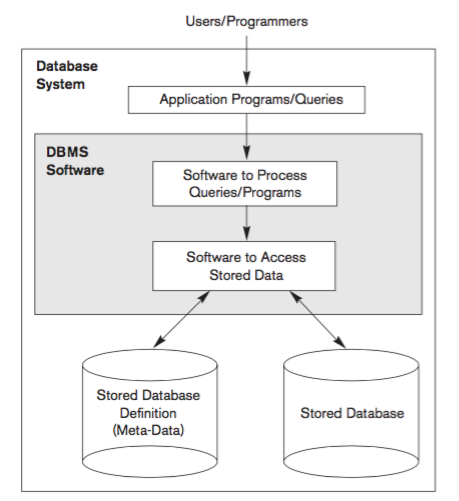
\includegraphics[scale=0.4]{chap1-1.png}
    \caption{A simplified database system environment}
    \label{fig:databaseSystem}
\end{figure}

\section{Characteristics of the Database Approach}

In \textbf{file processing}, each user defines and implements the files needed for a specific software application as part of programming the application. There is \textbf{redundancy} because each user maintains separate files. Moreover, if someone writes to a file and then shutdowns the system, there is no guarantee that the data have been written.\\

In the \textbf{database approach}, a single repository maintains data that is defined once and then can be accessed by various users.\\

\textbf{Main differences between databases and files:}
\begin{itemize}
    \item \textbf{Self-describing} nature of a database system
    \item \textbf{Insulation} between programs and data, and data abstraction
    \item Support of multiple \textbf{views} of data
    \item Sharing of data and \textbf{multi-user} transaction processing
\end{itemize}

\subsection{Self-describing nature}
The database system contains a complete definition of the database structure and constraints (its own model). It is stored in the DBMS catalog and is called the \textbf{meta-data}. The DBMS catalog also contains information about the structure of each file, the type and storage format of each data item and various constraints on the data. \textbf{NOSQL} systems do not require meta-data because they contain self-describing data that include the names and values together in one file.\\

File processing software can only access files with a specific structure. Whereas DBMS can access diverse databases by extracting the database definitions from the catalog. Moreover, the model of data is hardcoded. So there might be problems if the program is lost.\\

In files, there is a tight coupling between programs and physical data organization. If one of them changes, the other one must change too. The files and the data structure are \textbf{coupled}, it is bad.\\

\textbf{Coupling} happens when two things are strongly dependent. If one of them is broken, the system formed by those two things is broken too.

\subsection{Insulation between programs and data, and data abstraction}

The structure of data files is stored in the DBMS catalog, separately from the access programs. So a change to the structure does not always require to rewrite the program. It is called \textbf{program-data independence}. It is important to be able to change things (add a field, reorganize file, ..) without breaking everything (\textbf{management of changes}).\\

In some database systems, users can define \textbf{operations} (functions) that can be called regardless of how they are implemented. It is called \textbf{program-operation independence}.\\

Those two characteristics are allowed thanks to \textbf{data abstraction}. The DBMS provides \textbf{conceptual representation} without many details of how the data is stored or how the operations are implemented. A \textbf{data model} is a kind of data abstraction that is used to provide this conceptual representation.\\

The \textbf{conceptual schema} (neutral view) is between the external and the internal schemes.

\begin{figure}[!h]
    \centering
    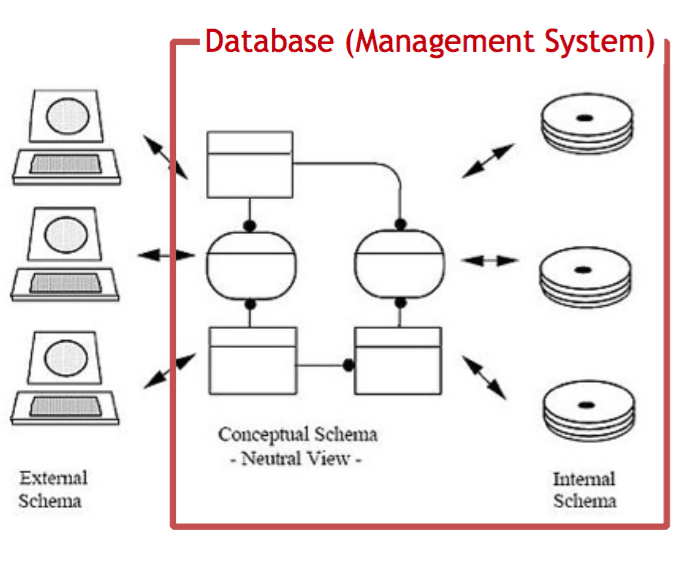
\includegraphics[scale=0.4]{chap1-2.png}
    \caption{Three schema architecture}
    \label{fig:architecture-1}
\end{figure}

Changes of data structures at the physical level (internal schema: disk) should be kept transparent at the logical level (external schema: user, programs).

\subsection{Support of Multiple Views of the Data}
A database has many types of users, each of whom may require a different perspective or view of the database. It can be a subset of the database or virtual data that is not stored.\\

Files have low level from an information standpoint.

\subsection{Sharing of Data and Multiuser Transaction Processing}

A multi-users DBMS must allow several users to access the database at the same time. There must be a \textbf{concurrency control} software to ensure that several users trying to update the same data do it in a controlled manner. These types of applications are often called \textbf{online transactions processing} (OLTP).\\

A relational database has a declarative query language. It describes what we want to do, not how (and it doesn't describe the control flow either).

A \textbf{transaction} is an executing program or process that includes one or more database accesses (reading or updating). If a transaction is executed completely, it is supposed to execute a logically correct database access.\\

It must also respect the \textbf{ACID} specification. They guarantee that concurrent databases transactions are processed reliably:\\

\begin{itemize}
    \item \textbf{Atomicity} : Either all database operations in a transaction are executed or none are.
    \item \textbf{Consistency}: Gives the correct answer. There are rules (invariants) that must always be true. For example, the value of $x$ must be in the interval [4,100]. It ensures that the database always goes from one valid state to another.
    \item \textbf{Isolation} Each transaction appears to execute in isolation from other transactions. Guarantee that even if many users use the database either one user see the other transactions because they are finished or he doesn't see them. The partial effects are invisible before the commit.
    \item \textbf{Durable}: If the system tells us that some data is stored after a commit, we can reboot it and it will still be there.
\end{itemize}

With files, it is hard to manage concurrent updates and failures. For example if several users want to read or write at the same time or if the system gets unplugged.

\section{Advantages of Using the DBMS Approach}
\subsection{Controlling redundancy}

Redundancy can cause several problems:

\begin{itemize}
    \item \textbf{Duplication of effort}: A single logical update must be performed several times (once for each file where this data is recorded).
    \item \textbf{Storage space wasted}
    \item \textbf{Data may become inconsistent}: it may happen if an update is not applied to all the files or different data can be written
\end{itemize}

\textbf{Data normalization} ensures consistency and saves storage space. However \textbf{controlled redundancy} can be used to improve performances (for example storing the student's id, course's id and grade in one summary table). The redundancy can be controlled with constraints and foreign keys to avoid inconsistency.

\subsection{Restricting unauthorized access}

Restrict the data that an user can access or the operations that he can perform. Users and user groups have accounts protected by passwords. The DBMS should provide a security and authorization subsystem to create accounts and specify restrictions. 

\subsection{Providing Persistent Storage for Program Objects}

Databases can be used to provide \textbf{persistent storage} for program objects and data structures. This is one of the main reasons for \textbf{object-oriented database systems}. It is easier and safer than storing the objects in the file with a specific format and then having to parse it.

\subsection{Providing Storage Structures and Search Techniques for Efficient Query Processing}

Database systems must be able to efficiently execute queries and updates. The DBMS must provide specialized data structures and search techniques to speed up the search on disk. Auxiliary files called \textbf{indexes} are used for this purpose. The DBMS often has a \textbf{buffering} or \textbf{caching} module.\\

The \textbf{query processing and optimization} module is responsible for choosing an efficient query execution plan for each query. The choice of which index to create and maintain is part of the physical database design and tuning.

\subsection{Providing Backup and Recovery}

A DBMS must provide facilities for recovering from hardware or software failures. For example, if the computer system fails in the middle of an update transaction, the recovery subsystem is responsible for making sure that the database is restored to the state it was in before the transaction started executing.

\subsection{Providing Multiple User Interfaces}

A DBMS should provide a variety of user interfaces (apps for mobile users, query languages, programming interfaces ...).

\subsection{Representing Complex Relationships among Data}

A DBMS must be able to represent complex relationships among data, to define new relationships as they arise and to retrieve and update related data easily and efficiently. 

\subsection{Enforcing integrity constraints}

Most databases have \textbf{integrity constraints} that must hold for the data. A DBMS should provide capabilities for defining and enforcing these constraints. 

\textbf{Examples of integrity constraints}:

\begin{itemize}
    \item Data type for each data item (ex. name must be a string of no more than 30 letters)
    \item Referential integrity constraint (foreign key)
    \item Key or uniqueness constraint
\end{itemize}

Constraints that aren't checked automatically and that must be checked by update programs or at the time of data entry are called \textbf{business rules}. Rules that pertain to a specific data model are called \textbf{inherent rules}.

\subsection{Permitting Inferencing and Actions Using Rules and Triggers}

\textbf{Deductive database systems} provides capabilities for defining deduction rules for inferencing new information from the stored facts. For example there might be rules to determine all students on probation. \\

A \textbf{trigger} is a form of rule activated by updates to the table, which results in performing some additional operations to some other tables.\\

\textbf{Stored procedures} are more involved procedures to enforce rules. They are part of the overall database definition and are invoked when some conditions are met. \\

\textbf{Active database systems} provide active rules that can automatically initiate actions when certain events and conditions occur.

\subsection{Additional implications of using the database approach}

\begin{itemize}
    \item \textbf{Potential for enforcing standards}: names and formats of data elements, display formats, reports structures, terminology ...
    \item \textbf{Reduced application development time}: once a database is up and running, less time is required to create new applications using DBMS facilities.
    \item \textbf{Flexibility}: it may be necessary to change the structure of a database as requirements change. Modern DBMSs allow certain types of evolutionary changes to the structure of the database without affecting the stored data and the existing application programs.
    \item \textbf{Availability of up-to-date information}: a DBMS makes the database available to all users. Every user can see the updates immediately. 
    \item \textbf{Economies of scale} : the DBMS approach permits consolidation of data and applications
\end{itemize}

\section{A brief history of database applications}

One of the main problems with early database systems was the intermixing of conceptual relationships with the physical storage and placement on the disk. They did not provide enough \textbf{data abstraction} and \textbf{program-data independence} capacities. New queries that required a different storage organization for efficient processing where difficult to implement. \\

\textbf{Relational databases} were originally proposed to separate the physical storage of data from its conceptual representation and to provide a mathematical foundation for data representation and querying. They use relations that are represented by tables. A relation is only used to give meaning to the stored data.\\

The relational model says nothing about:\\

\begin{itemize}
    \item How relations are stored
    \item How data is to be distributed over nodes/servers
    \item What data types are available
    \item How tuples are ordered, indexed
\end{itemize}

\section{When not to use a DBMS}

\textbf{Overhead costs of using a DBMS}:

\begin{itemize}
    \item High initial investment in hardware, software and training
    \item Generality that it provides for defining and processing data
    \item Overhead for providing security, concurrency control, recovery and integrity functions
\end{itemize}

It might not be desirable to use a DBMS in the following situations:\\

\begin{itemize}
    \item Simple, well-defined database applications that are not expected to change at all
    \item Stringent, real-time requirements for some application programs that may not be met because of DBMS overhead
    \item Embedded systems with limited storage capacity, where a general-purpose DBMS would not fit
    \item No multiple-user access to data
\end{itemize}

\section{Main causes for NoSQL and NewSQL}

\begin{itemize}
    \item \textbf{Big data}: too much data for relational implementation to handle the load
    \item \textbf{Relational pack overused}: many software simply require storage, not all software are multi-user and sometimes we don't need to have the ACID properties.
    \item \textbf{Requires upfront thinking}: the current motto is \textbf{do and then think}
    \item \textbf{SQL has many flaws}: for example lack of user-defined data types
    \item \textbf{Data independence}: it can be achieved by other means when the data layer offers a low-level quality of service.
    \item The relational model is about working with \textbf{high-level abstractions} (for weak coupling, long-term maintenance, meeting the needs of every user even the ones we don't know yet). No one is favoured regarding data access. It is not compatible with the way most new businesses want to work
\end{itemize}

\section{Summary}

The keys messages are the following:\\

\begin{itemize}
    \item \textbf{Database definition}: focus on information, not only storage
    \item \textbf{Data independence}: weak coupling for easier maintenance
    \item \textbf{High-level specification}: behavioral guarantees for meeting requirements
    \item \textbf{Declarative vs procedurale}: Information aims at being queried
\end{itemize}

\textbf{\textcolor{red}{Examples of exam question}}:
\begin{itemize}
    \item Give two main ideas for the database (example: decoupling and ACID)
    \item Why were databases invented with hard disk (because they provide random accesses, on tapes there were only sequential accesses).
    \item Give 5 examples of physical changes that don't affect the external schema 
    \begin{itemize}
        \item Encoding
        \item Different file organization or storage structures
        \item Storage devices (hard-disk or SSD)
        \item Indexing strategy (hash index, B-tree ..)
        \item Switching from one access method to another
        \item Exact location of data on disk
        \item Compression
        \item Splitting
        \item Merging of records
    \end{itemize}

\end{itemize}

\chapter{Database System Concepts and Architecture (Chapter 2)}


\section{Data Models, Schemas, and Instances}

A \textbf{client module} handles user interaction and provides user-friendly interfaces. Whereas a \textbf{server module} handles data storage, access, search and other functions.\\

Databases provide \textbf{data abstraction} (suppression of details of data organization and storage and highlighting of essential features). A \textbf{data model} is a collection of concepts that can be used to describe the structure of a database. They also include a set of \textbf{basic operations}.\\

The \textbf{dynamic aspect} or \textbf{behavior} is a set of user-defined operations that are allowed on the database objects (for example compute GPA).\\

\subsection{Categories of Data Models}

\textbf{High-level} or \textbf{conceptual data models} provide concepts that are close to the way many users perceive data. \textbf{Low-level} or \textbf{physical data models} provide concepts that describe the details of how data is stored.\\

Conceptual data models use different concepts:\\

\begin{itemize}
    \item \textbf{Entity}: represents a real-world object or concept (such as an employee or project)
    \item \textbf{Attribute}: represents some property of interest that further describes the entity
    \item \textbf{Relationships}: represents association among the entities. 
\end{itemize}

\subsection{Schemas, Instances, and Database State}

The \textbf{database schema} is the description of the database. It is specified during database design and is not expected to change frequently. A \textbf{schema diagram} is a displayed schema of the database.\\

The database state at a particular moment in time is called a \textbf{database state} or \textbf{snapshot}. 

\section{Three-schema architecture and data independence}

This kind of schema helps to achieve the three following characteristics:\\

\begin{itemize}
    \item Use of a catalog to store the database schema and make it self-describing
    \item Insulation of programs and data
    \item Support of multiple user views
\end{itemize}

\subsection{The three-schema architecture}

The goal is to separate the user applications from the physical database. Schemas can be defined at the following three levels:\\

\begin{figure}[!h]
    \centering
    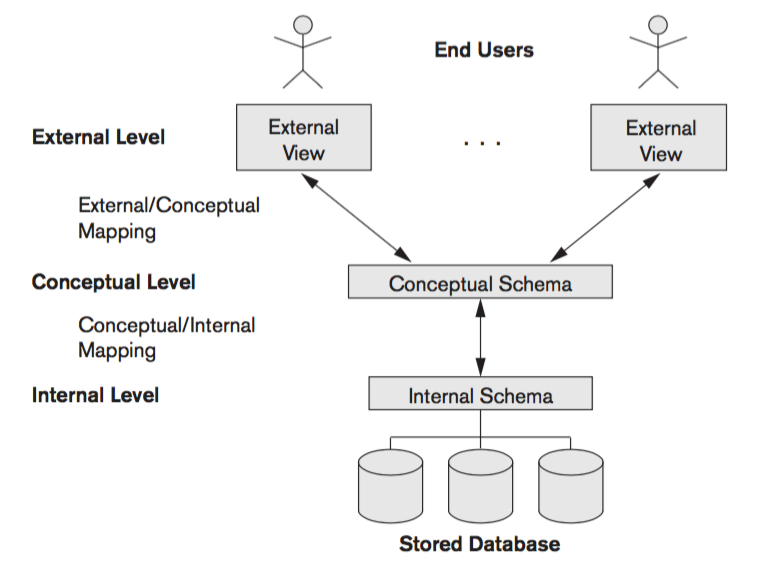
\includegraphics[scale=0.4]{chap2-1.png}
    \caption{Three schema architecture}
    \label{fig:architecture-2}
\end{figure}

\begin{itemize}
    \item \textbf{The internal level} has an \textbf{internal schema} which describes the physical storage structure of the database. It describes the complete details of data storage and access paths.
    \item \textbf{The conceptual level} describes the structure of the whole database for a community of users. It hides the details of physical storage structures and focus on describing entities, attributes, relationships, user operations and constraints.
    \item \textbf{The external or view level} includes a number of external schemas. They describe the views of different user groups.
\end{itemize}

In this architecture, each user group refers to its own external schema. The DBMS must transform a request specified on an external schema into a request against the conceptual schema, and then into a request on the internal schema. When the data is extracted, it must be reformatted to match the user's external view. The processes of transforming requests and results between levels are called \textbf{mappings}.

\subsection{Data independence}

\textbf{Data independence} is the capacity to change the schema at one level without having to change it at the next higher level. There are two types of data independence:\\

\begin{itemize}
    \item \textbf{Logical data independence}: capacity to change the conceptual schema without having to change external schemas or application programs. Only the view definitions and the mappings need to be changed.
    \item \textbf{Physical data independence}: capacity to change the internal schema without having to change the conceptual schema (exact location of data on disk, and hardware details of storage encoding, placement, compression, splitting, merging of records) 
\end{itemize}

Logical data independence is harder to achieve because it allows structural and constraint changes without affecting application programs.

\section{Database languages and interfaces}

\subsection{DBMS languages}

\textbf{Types of languages}:\\

\begin{itemize}
    \item \textbf{Data Definition Language}: used to define both the conceptual and internal schemas
    \item \textbf{Storage Definition Language} : used to specify the internal schema
    \item \textbf{View Definition Language}: used to specify user views and their mappings to the conceptual schema
    \item \textbf{Data Manipulation Language}: used for retrieval, insertion, deletion and update
\end{itemize}

However in current DBMS those languages aren't considered distinct. SQL is a combination of DDL, VDL and DML.\\

There are two types of DML:\\

\begin{itemize}
    \item \textbf{High level} or \textbf{non procedural}: used on its own to specify complex database operations concisely. They can be entered from a terminal. They can specify and retrieve many records in a single DML statement (\textbf{set-at-a-time})
    \item \textbf{Low level} or \textbf{procedural}: must be embedded in a general-purpose programming language. This type of DML typically retrieves individual records or objects from the database and processes each separately (\textbf{record-at-a-time})
\end{itemize}


\chapter{Data Modeling Using the Entity–Relationship (ER) Model (Chapter 3)}  



    Object modeling methodologies such as Unified Modeling Language (UML) are becoming increasingly popular in both database and software design. These methodologies go beyond database design to specify detailed design of software modules and their interactions using various types of diagrams. Class diagrams are similar in many ways to the ER diagrams. In class diagrams, operations on objects are specified, in addition to specifying the database schema structure. Operations can be used to specify the functional requirements during database design.

\section{Using High-Level Conceptual Data Models for Database Design}
    
    \begin{figure}
        \centering
        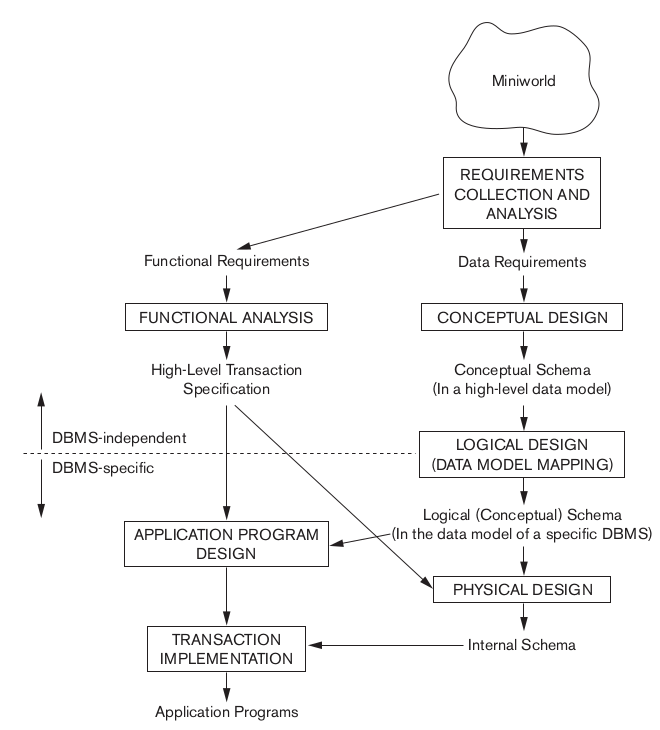
\includegraphics[scale=0.4]{chap3-1}
        \caption{A simplified diagram to illustrate the main phases of database design.}
        \label{fig:chap3-1}
    \end{figure}
    
    \textbf{Conceptual schema}: concise description of the data requirements of the users and includes detailed descriptions of the entity types, relationships, and constraints; these are expressed using the concepts provided by the high-level data model.
    
    \textbf{Logical design} or \textbf{data model mapping}: actual implementation of the database using
    a commercial DBMS, using an implementation data model - such as the relational (SQL) model - so the conceptual schema is transformed from the high-level data model into the implementation data model.
    
    \textbf{Physical design} phase: specify the internal storage structures, file organizations, indexes, access paths, and physical design parameters for the database files

\section{Entity Types, Entity Sets, Attributes,and Keys}
    \subsection{Entities and Attributes}
    \begin{itemize}
        \item \textbf{Entity}: thing or object in the real world with an independent existence
    May be an object with a physical existence (a particular person, car, house, or employee) or an object with a conceptual existence (a company, a job, or a university course). 
        \item \textbf{Attributes}: particular properties that describe an entity. 
    \end{itemize}
    
    \subsubsection{Attribute types}
    \begin{itemize}
        \item \textbf{Composite} attributes can be divided into smaller subparts (which can also be composite attributes (ex:street\_address $\rightarrow$ number, street)), which represent more basic attributes with independent meanings (ex: an address $\rightarrow$ street\_address, zip, city)
        \item \textbf{Simple} or \textbf{atomic} attributes cannot be divided.
        \item \textbf{Single-valued} attributes have a single value for a particular entity
        \item \textbf{Multivalued} attributes that can have a \textbf{set of values} or \textbf{domain} for the same entity (ex: colors of a car) (not represented on ER diagrams)
        \item \textbf{Derived} attributes can be determined by using one or more \textbf{stored} attributes or related entities (ex: \# of employees)
        \item \textbf{NULL values}: a particular entity may not have an applicable value (not applicable) or we don't know the value of that attribute (missing)
        \item \textbf{Complex} attributes are grouped composite attributes whose components are displayed using parentheses (), separated by commas and displaying multivalued attributes between braces \{\}
    \end{itemize}


\section{Entity Types, Entity Sets, Keys, and Value Sets}
\begin{itemize}
    \item \textbf{Entity type}: defines a collection (or set) of entities that have the same attributes (ex: Employee). Each entity type in the database is described by its name and attributes.
    
    \item \textbf{Entity set} or \textbf{entity collection}: collection of all entities of a particular entity type in the database, also called the extension of the entity type. (the entity set is usually referred to using the same name as the entity type, even though they are two separate concepts)
    
    \item An entity type describes the \textbf{schema} or \textbf{intension} for a set of entities that share the same structure. 
    
    \item \textbf{Uniqueness constraint} on attributes (or \textbf{key}). These attributes can be used to identify each entity uniquely. 
    \item \textbf{Composite key}: Several attributes together can form a key: the combination of the attribute values must then be distinct for each entity. To represent this in the ER model, define a composite attribute and designate it as a key attribute of the entity type. Composite keys must be \textbf{minimal}; that is, all component attributes must be included in the composite attribute to have the uniqueness property

    \begin{figure}
        \centering
        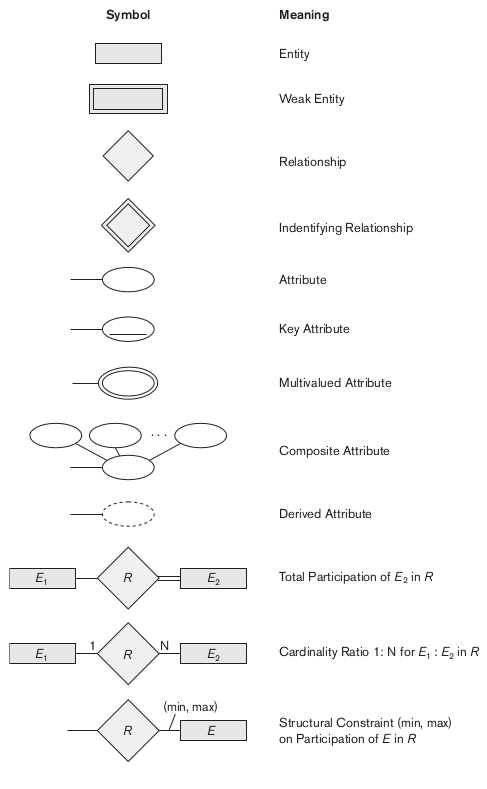
\includegraphics[scale=0.4]{chap3-14}
        \caption{Summary of the notation for ER diagrams.}
        \label{fig:chap3-14}
    \end{figure}
    
    \item \textbf{Weak entity type}: Entity type that has no key.


\section{Relationship Types, Relationship Sets, Roles, and Structural Constraints}
    \subsection{Relationship Types, Sets, and Instances}
    \paragraph{Book}
    A \textbf{relationship type} $R$ among $n$ entity types $E_1, E_2, ...E_n$ defines a set of associations—or a \textbf{relationship set}—among entities from these entity types. Both are referred by the same name $R$.
    
    Mathematically, the \textbf{relationship set} R is a set of \textbf{relationship instances} $r_i$, where each $r_i$ associates $n$ individual entities $(e_1,..,e_n)$ and each entity $e_j$ in $r_i$ is a member of the entity set $E_j$ ($1\leq j\leq n)$

    \paragraph{Slides}
    A \textbf{relation} represents the extension of some $n$-adic predicate P by having a body consisting of every $n$-tuple that satisfies P

    The corresponding mathematical intension could be: $$\{ < s, c > | \text{Student s is enrolled on course c} \}$$
    
    \begin{itemize}
        \item \textbf{Predicate}: The meaning of a certain kind of sentence, but often used (conveniently) to refer to the sentence itself.
        \item \textbf{Intension} of a predicate: its meaning (loosely speaking)
        \item \textbf{Extension} of a predicate: all the instantiations that are (believed to be) true.
        \item \textbf{Substitution}: replace a parameter by a designator
        \item \textbf{Instantiation}: substitution of all the parameters, yielding a proposition.
    \end{itemize}

    \paragraph{DEE and DUM}
    Relations corresponding to :
    \begin{itemize}
        \item $\{< > | 2 < 1\}$ : DUM (false)
        \item $\{< > | 2 > 1\}$ : DEE (true)
    \end{itemize}
    
    \begin{itemize}
        \item DUM is the relation that has no attributes and no tuples. It plays the role of False.
        \item DEE is the relation that has no attributes and a single tuple. It plays the role of True.
    \end{itemize}



    \subsection{Relationship Degree, Role Names, and Recursive Relationships}

    \begin{itemize}
        \item \textbf{Degree} of a relationship type: number of participating entity types (ex: binary, ternary, ...)
         \item \textbf{Recursive relationships} or \textbf{self-referencing relationships}: relationship in which the same entity type participates more than once but in different roles. (ex: employee and supervisor, which are both of type EMPLOYEE)
    \end{itemize}

    \subsection{Constraints on Binary Relationship Types}
    
    \begin{itemize}
        \item \textbf{Cardinality ratio}: specifies the \emph{maximum} number of relationship instances that an entity can participate in (ex: 1:1, 1:N, N:1, M:N)
        \item \textbf{Participation constraint} or \textbf{minimum cardinality constraint}: specifies the \emph{minimum} number of relationship instances that each entity can participate in. 2 kinds : total (or existence dependency) (\emph{double line}) and partial(\emph{single line}).
    \end{itemize}
    
    \subsection{Attributes of Relationship Types}
    Relationship types can also have attributes, similar to those of entity types. For example, to record the number of hours per week that a particular employee works on a particular project.
    
    \begin{itemize}
        \item Attributes of a 1:1 relationship type can be migrated to one of the participating entities
        \item Attributes of a 1:N relationship type can be migrated only to the entity type on the N-side
        \item Attributes of a M:N relationship type cannot be migrated and must have a dedicated relationship
    \end{itemize}
    
    Other (more precise) notation exists with (min, max)
    
    
\section{Weak entity types}

Entities belonging to a \textbf{weak} entity type are identified by being related(\textbf{identifying relationship}) to specific entities from another entity type(called \textbf{identifying} or \textbf{owner}) in combination with one of their attribute values.

A weak entity type always has a \emph{total participation constraint} with respect to its identifying relationship because a weak entity cannot be identified without an owner entity.

\begin{itemize}
    \item \textbf{Partial key}: attribute (may be composite, or all the weak entity's attributes) that can uniquely identify weak entities that are related to the same owner entity
\end{itemize}

\end{itemize}




\chapter{The Enhanced Entity-Relation (EER) Model (Chapter 4)}

\section{Subclasses, Superclasses, and Inheritance}

The EER model adds the following concepts:\\

\begin{itemize}
    \item \textbf{subclass} and \textbf{superclass}
    \item \textbf{specialization} and \textbf{generalization}
    \item \textbf{category} or \textbf{union type} (used to represent a collection of entities = union of objects of different entity types)
    \item \textbf{attribute and relationship inheritance}
\end{itemize}

A \textbf{subtype} or \textbf{subclass} of an entity type are used to represent subgroupings or subtypes of an entity that are meaningful. They need to be represented explicitly because of their significance to the database application. For example $EMPLOYEE$ can be distinguished in $SECRETARY$, $ENGINEER$ and $TECHNICIAN$.\\

The set in each of the subgroupings is a subset of the entities that belong to the $EMPLOYEE$ entity set. $EMPLOYEE$ is called the \textbf{superclass} or \textbf{supertype}. The relation between a superclass and a subclass is called \textbf{class/subclass relationship}. An entity can be a member of any number of subclasses. The EER notation is given on figure \ref{fig:subclasses}.\\

\begin{figure}[!h]
    \centering
    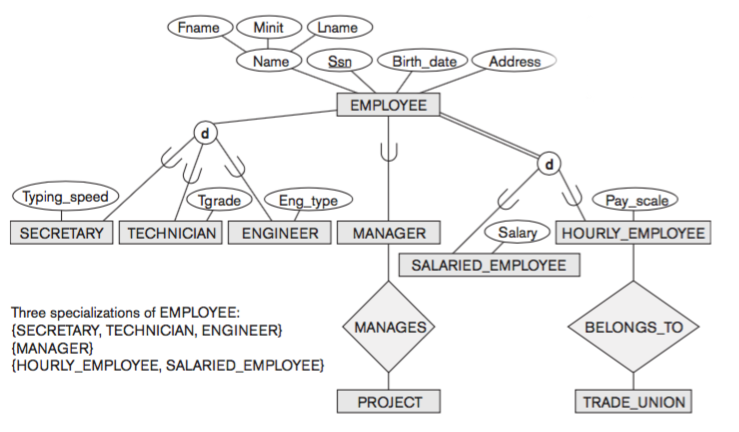
\includegraphics[scale=0.4]{chap4-1.png}
    \caption{EER notation to represent subclasses and specialization}
    \label{fig:subclasses}
\end{figure}

The \textbf{type} of an entity is defined by the attributes that it possesses and the relationship types in which it participates.\\

An entity that is a member of a subclass \textbf{inherits} all the attributes of the entity as a member of the superclass (= \textbf{type inheritance}). It also inherits all the relationships in which the superclass participates. A subclass can also have specific attributes and relationships.

\section{Specialization and generalization}

\subsection{Specialization}

\textbf{Specialization} is the process of defining a set of subclasses of an entity type. This set of subclasses is defined on the basis of some distinguishing characteristics of the entities in the superclass. There can be several specializations of the same entity type based based on different distinguishing characteristics.
Figure \ref{fig:subclasses} shows the EER representation. The subset symbols on each line indicate the direction of the superclass/subclass relationship.\\

An entity that belongs to a subclass represents the same real-world entity as the corresponding entity in the superclass.\\

There are two main reasons for including class/subclass relationships and specializations:\\

\begin{itemize}
    \item Certain attributes may apply to some but not all entities of the superclass entity type. A subclass is defined in order to group the entities to which these attributes apply.
    \item Some relationship types may be participated in only by entities that are members of the subclass. For example, only $HOURLY\_EMPLOYEE$ are related to the entity type $TRADE\_UNION$ by the relation $BELONGS\_TO$.
\end{itemize}
    
\subsection{Generalization}

\textbf{Generalization} is the process of suppressing the differences among several entity types (by identifying their common features) to generalize them into a \textbf{superclass}. The original entity types are special subclasses. For example $CAR$ and $TRUCK$ can be generalized in $VEHICLE$.

\section{Constraints and characteristics of specialization and generalization hierarchies}

\subsection{Constraints on Specialization and Generalization}

\textbf{Predicate-defined subclasses} are the ones for which we can determine the entities that will become members of each subclass by placing a condition on the value of some attribute of the superclass\\

\begin{figure}[!h]
    \centering
    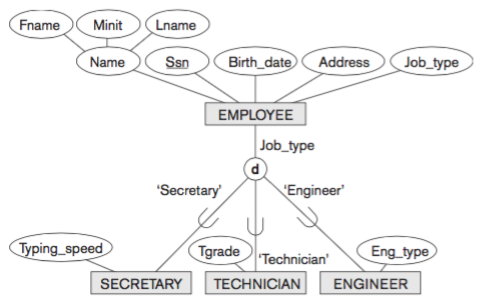
\includegraphics[scale=0.4]{chap4-2.png}
    \caption{Attribute-defined specialization on Job\_type}
    \label{fig:predicate}
\end{figure}

If all subclasses have their membership condition on the same attribute of the superclass, we call it an \textbf{attribute-defined} specialization and the attribute is called the \textbf{defining attribute} (cfr. figure \ref{fig:predicate}).\\

When there is no condition to determine membership in a subclass, it is called an \textbf{user-defined} subclass (membership determined by the user).\\

The \textbf{disjointness constraint} specifies that the subclasses of a specialization must be disjoint sets. An entity can be a member of at most one subclass. The representation is shown on figure \ref{fig:predicate} (the $d$ in the circle). Otherwise, the sets of entities may be \textbf{overlapping}. It is represented with a $o$ in a circle and not a $d$.\\

\textbf{A total (or completeness) specialization constraint} specifies that every entity in the superclass must be a member of at least one subclass in the specialization. It is represented by using a double line to connect the superclass to the circle (cfr. figure \ref{fig:subclasses}). A single line is used for \textbf{partial participation} which allows an entity not to belong to any subclass.\\

The \textbf{disjointness} and \textbf{completeness} constraints are independent.

\textbf{Rules for insertion and deletion}:\\

\begin{itemize}
    \item \textbf{Deleting} an entity from a superclass implies that it is automatically deleted from all the subclasses to which it belongs.
    \item \textbf{Inserting} an entity in a superclass implies that the entity is mandatorily inserted in all predicate-defined  subclasses for which the entity satisfies the defining predicate
    \item \textbf{Inserting} an entity in a superclass of a total specialization implies that the entity is mandatorily inserted in at least one of the subclasses
\end{itemize}

\subsection{Specialization and Generalization Hierarchies and Lattices}

A subclass may have further subclasses specified on it, forming a hierarchy or a lattice of specializations.\\

\begin{itemize}
    \item \textbf{Specialization hierarchy}: each subclass has only one parent (\textbf{tree} structure)
    \item \textbf{Specialization lattice}: a subclass can have several parents (cfr. figure \ref{fig:lattice})
\end{itemize}

In such a specialization lattice or hierarchy, a subclass inherits the attributes of all its predecessor superclasses.\\

\begin{figure}[!h]
    \centering
    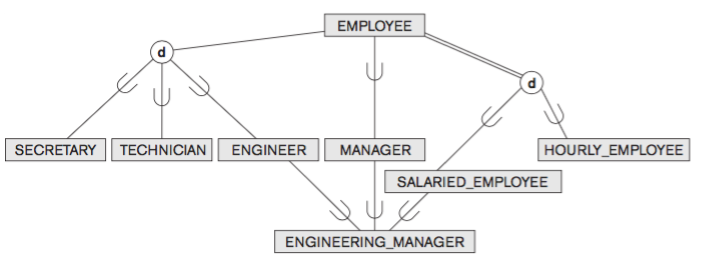
\includegraphics[scale=0.4]{chap4-3.png}
    \caption{A specialization lattice}
    \label{fig:lattice}
\end{figure}

A \textbf{shared subclass} is a subclass with more than one parent (\textbf{multiple inheritance}).\\

Some models and languages don't allow multiple inheritance and/or multiple types.

\subsection{Utilizing Specialization and Generalization in Refining Conceptual Schemas}

\textbf{Top-down conceptual refinement} is the process of starting with one entity type and then specializing it into several subclasses.

\textbf{Bottom-up conceptual synthesis} is the contrary. First start with the last level of subclassess and then generalize them. 

\section{Modeling of UNION Types Using Categories}

An \textbf{union type} or \textbf{category} is a subclass that represents a collection of entities from different entity types. For example if a vehicle can have three types of owner $PERSON$, $BANK$ or $COMPANY$, it is possible to create a category $OWNER$ that is a subclass of the union of the three entity sets (cfr. figure \ref{fig:category}). \\

\begin{figure}[!h]
    \centering
    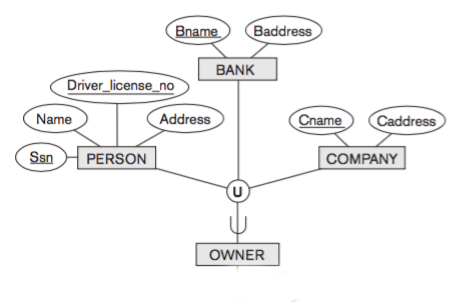
\includegraphics[scale=0.4]{chap4-4.png}
    \caption{Category OWNER}
    \label{fig:category}
\end{figure}

\textbf{Difference between a category and a shared subclass}:\\

\begin{itemize}
    \item \textbf{Category}: subset of the \textbf{union} of its superclasses. An entity belonging to a category must exist in only one of the superclasses. It inherits the attributes of the superclass to which it belongs.
    \item \textbf{Shared class}: subclass of each of the superclass. So an entity that is a member of a shared class must exists in all the superclasses' collections. Its entity set is a subset of the \textbf{intersection} of the entity sets. It inherits the attributes of all the superclasses
\end{itemize}

A \textbf{total} category holds the union of all the entities in its superclasses. It is represented with a double line connecting the category and the circle. A \textbf{partial} category holds a subset of the union.

\section{Design Choices and Formal Definitions}

\subsection{Design choices}

\textbf{Guidelines to guide the design process}:\\

\begin{itemize}
    \item Represent only those subclasses that are necessary to avoid extreme cluttering of the conceptual schema
    \item If a subclass has few specific (local) attributes and no specific relationships, it can be merged into the superclass (possibly add a type attribute).
    \item If all the subclasses of a specialization have few specific attributes and no specific relationships, they can be merged into the superclass and replaced with one or more type attributes
    \item Union types and categories should be avoided unless really necessary.
    \item The choice of disjoint/overlapping and total/partial depends on the miniworld being modeled.
\end{itemize}

\subsection{Formal Definitions for the EER Model Concepts}

\textbf{Definitions}:\\

\begin{itemize}
    \item \textbf{Class}: defines a type of entity and represents a set or collection of entities of that type.
    
    \item \textbf{Subclass}: class whose entities must always be a subset of the entities in another class called the \textbf{superclass}
    
    \item \textbf{Specialization}: set of subclasses Z=$\big\{$S1,S2,..,Sn$\big\}$ that have the same super class G called the \textbf{Generalized entity type} (or \textbf{superclass}). 
    
    The specialization is said to be \textbf{total} if $\bigcup_{i=1}^n S_i$ = G. 
    
    Z is \textbf{disjoint} if we have $S_i \bigcap S_j$ = $\emptyset$ for i$\neq$j. Otherwise it is \textbf{overlapping}
    
    \item \textbf{Predicate defined subclass}: if a predicate on the attributes is used to specify which entities are members of the subclass.
    
    Otherwise it is \textbf{user defined}
    
    \item \textbf{Attribute-defined specialization} : if a predicate A = $c_i$ (with A an attribute of the superclass and $c_i$ a constant from the domain of A) is used to specify membership in each subclass $S_i$.
    
    \item \textbf{Category}: class T that is a subset of the union of n defining superclass $D_1$ .. $D_n$. So we have T $\subseteq$ ($D_1$ $\cup$ .. $\cup$ $D_n$).
    
    A predicate $p_i$ on the attributes of $D_i$ can be used to specify the members of each $D_i$ that are members of T.
    
    T $\subseteq$ ($D_{1}[p_1]$ $\cup$ .. $\cup$ $D_{n}[p_n]$).
 \end{itemize}
 
 The definition of relationship type must be extended to allow any class to participate in a relationship (replace the word entity type by class in the definition).
 
 %\section{Data Abstraction, Knowledge Representation, and Ontology Concepts}
 
 %\textcolor{red}{\textbf{TODO}} But not really important I think ...

\chapter{Basic SQL (Chapter 6)}
\section{SQL Data Definition and Data Types}
\textit{SQL} uses specific terms to talk about formal relational model terms:
\begin{itemize}
    \item \textit{Table} $\rightarrow$ \textit{Relation};
    \item \textit{Row} $\rightarrow$ \textit{Tuple};
    \item \textit{Column} $\rightarrow$ \textit{Attribute}.
\end{itemize}
One of the main \textit{SQL} command is \textbf{CREATE} with this you can create \textit{schemas}, \textit{tables}, \textit{types}, \textit{domains}, \textit{views}, \textit{assertions} and triggers.
\subsection{Schema and Catalog Concepts in SQL}
Before \textit{SQL2} the concept of a relational database schema wasn't include, all the table were in the same schema.
An \textit{SQL} schema is identified by a schema name and includes an authorization identifier, as well as descriptors for each element in the schema. Schema elements include \textit{tables}, \textit{types}, \textit{constraints}, \textit{views}, \textit{domains}, etc.
We use the command \textbf{CREATE SCHEMA}, which can include all the schema elements definitions, to create a schema\footnote{Note that each statement in SQL ends with a semicolon.}. A catalog correspond to a named collection of schema.
\subsection{The CREATE TABLE Command in SQL}
The \textbf{CREATE TABLE} command is used to specify a new relation by giving it a name and specifying its attributes and initial constraints. The attributes are specified first, and each attribute is given a name, a data type to specify its domain of values, and possibly attribute constraints (e.g \textbf{NOT NULL}). The key, entity integrity, and referential integrity constraints can be specified to, or can be added later\footnote{See next chapter.}. Typically, we implicitly tell the schema in which the relation will be created but it can also be implicit. \textbf{CREATE TABLE (SCHEMA\_NAME.)TABLE\_NAME}.

Base tables\footnote{different of \textbf{virtual tables}, see next chapter}, relation created through \textbf{CREATE TABLE}, are created and stored, with these actual rows, as a file by the DBMS.

Note that foreign key can make errors because of circular references or refers a table that didn't exist that can be corrected with the command \textbf{ALTER TABLE}.
\subsection{Attribute Data Types and Domains in SQL}
There are different basic type in \textit{SQL}:
\begin{itemize}
    \item \textbf{Numeric};
    \item \textbf{Character-string};
    \item \textbf{Bit-string};
    \item \textbf{Boolean};
    \item \textbf{Date}, \textbf{Time}, \textbf{Timestamp} (special type of string $\rightarrow$ easy cast for comparison).
\end{itemize}
 You can create your own type with the command \textbf{CREATE TYPE}.
\section{Specifying Constraints in SQL}
\subsection{Specifying Attribute Constraints and Attribute Defaults}
\textit{SQL} allows \textbf{NULL} so the first constraint is to restrict the utilization of \textbf{NULL} on attributes that can't be null(Implicit on the primary key). If a \textbf{NULL} value appears it can be changed by a default value: \textbf{NAME TYPE NOT NULL DEFAULT NEW$\_$VALUE}. Other type of constraints can be checked with \textbf{CHECK}(Boolean). It can also be used with \textbf{CREATE DOMAIN} statement. 
\subsection{Specifying Key and Referential Integrity Constraints}
There are specific clauses in \textbf{CREATE TABLE} to specify constraints on keys and referential integrity. The \textbf{PRIMARY KEY} clause specifies one or more attributes that make up the primary key of a relation. The \textbf{UNIQUE} clause specifies alternate (unique) keys, also known as candidate keys. Referential integrity is specified via the \textbf{FOREIGN KEY} clause a referential integrity constraint can be violated when tuples are inserted or deleted, or when a foreign key or primary key attribute value is updated. The default action that \textit{SQL} takes for an integrity violation is to reject the update operation that will cause a violation, which is known as the \textbf{RESTRICT} option. However, the schema designer can specify an alternative action to be taken by attaching a referential triggered action clause to any foreign key constraint. Other options are\textbf{SET NULL}, \textbf{CASCADE} (delete referencing tuples), \textbf{SET DEFAULT}, \textbf{ON DELETE} and \textbf{ON UPDATE}.
\subsection{Giving Names to Constraints}
The name is following the \textbf{CONSTRAINT} statement and must be unique. But it's optional.
\subsection{Specifying Constraints on Tuples Using CHECK}
Other table constraints can be added at the end of \textbf{CREATE TABLE} by adding \textbf{CHECK}, they are row-based constraints (apply on each row independently), that check each row when something is add or updated.
\section{Basic Retrieval Queries in SQL}
The basic statement to find information is the statement \textbf{SELECT}.
\textit{SQL} allow a table to have two or more identical tuples. Hence, in general, an \textit{SQL} table is not a set of tuples (because a set does not allow two identical members), rather, it is a multiset of tuples. Some \textit{SQL} relations are constrained to be sets because a key constraint has been declared or because the \textbf{DISTINCT} option has been used with the \textbf{SELECT} statement.
\subsection{The SELECT-FROM-WHERE Structure of Basic SQL Queries}
The basic aspect of an \textit{SQL} request is: \textbf{SELECT} $<$attribute list$>$ (called projection attributes) \textbf{FROM} $<$table list$>$ \textbf{WHERE} $<$condition$>$(called selection/join attributes);\footnote{Not equal in \textit{SQL} is "$<>$"} If there is no \textbf{WHERE} it test all the possible choices (corss product). 
\subsection{Ambiguous Attribute Names, Aliasing, Renaming, and Tuple Variables}
It is possible that different attributes has the same name if they are not in the same table, so we must qualify the attribute name bu prefixing the table of reference: \textbf{TABLE.ATTRIBUTE$\_$NAME}. Ambiguity can also append where we use the same relation multiple time in a single request, the solution is to rename the relation with \textbf{AS}: ... \textbf{FROM RELATION AS NEW$\_$NAME1, RELATION AS NEW$\_$NAME2 WHERE} ...
\subsection{Unspecified WHERE Clause and Use of the Asterisk}
If we want all attributes for a specific relation, we put * in the \textbf{SELECT statement}.
\subsection{Tables as Sets in SQL}
As we mentioned earlier, \textit{SQL} usually treats a table not as a set but rather as a multiset as duplicate tuples can appear more than once in a table, and in the result of a query. If we do want to eliminate duplicate tuples from the result of an \textit{SQL} query, we use the keyword \textbf{DISTINCT} in the \textbf{SELECT} clause. There are some operations on sets: \textbf{UNION}, \textbf{EXCEPT} and \textbf{INTERSECT}. Duplicate states are deleted in their results.
\subsection{Substring Pattern Matching and Arithmetic Operators}
You can use \textbf{LIKE} to make pattern matching. \% replaces an arbitrary number of zero or more characters, and the underscore replaces a single character.
\subsection{Ordering of Query Results}
\textit{SQL} allows the user to order the tuples in the result of a query by the values of one or more of the attributes that appear in the query result, by using the \textbf{ORDER BY} clause. Default value: ascending order of value, you can use \textbf{ASC} or \textbf{DESC} to change it.
\subsection{Discussion and Summary of Basic SQL Retrieval Queries}
\textbf{SELECT} $<$attribute list$>$
\textbf{FROM} $<$table list$>$ 
[ \textbf{WHERE} $<$condition$>$ ]
[ \textbf{ORDER BY} $<$attribute list$>$ ];
\section{INSERT, DELETE, and UPDATE Statements in SQL}
\subsection{The INSERT Command}
This is used to add a tuple in a relation. \textbf{INSERT INTO} table \textbf{VALUE} tuple (in the same order as define in the table).
We can also tell explicitly what we want to fill, the rest will be \textbf{NULL} or default value.
A DBMS that fully implements SQL should support and enforce all the integrity constraints that can be specified in the DDL
\subsection{The DELETE Command}
This is used to delete row in a relation. \textbf{DELETE FROM} table \textbf{WHERE} condition;
\subsection{The UPDATE Command}
This is used to update row in a relation. \textbf{UPDATE} table \textbf{SET} changements \textbf{WHERE} condition;
\section{Additional Features of SQL}
Not really interesting in my opinion.
\section{Summary}
\textit{SQL} is designed to be a comprehensive language that includes statements for data definition, queries, updates, constraint specification, and view definition. We discussed the following features of \textit{SQL} in this chapter: the data definition commands for creating tables, \textit{SQL} basic data types, commands for constraint specification, simple retrieval queries, and database update commands.

 


\chapter{More SQL: Complex Queries, Triggers, Views, and Schema Modification (Chapter 7)}
\section{More Complex SQL Retrieval Queries}
\subsection{Comparisons Involving NULL and Three-Valued Logic}
\textit{SQL} has some rules to manage \textbf{NULL} that can have three different interpretations:
\begin{itemize}
\item Unknown value;
\item Unavailable or withheld value;
\item Not applicable attribute.
\end{itemize}
It's often hard to detemine this interpretation. Each individual \textbf{NULL} is different. When we apply a comparison operation on a tuple which has a \textbf{NULL} value, the result is \textbf{UNKNOWN}. The figure \ref{7-1} show how logical operators are used with \textbf{UNKNOWN}:
\begin{figure}[H]
    \centering
    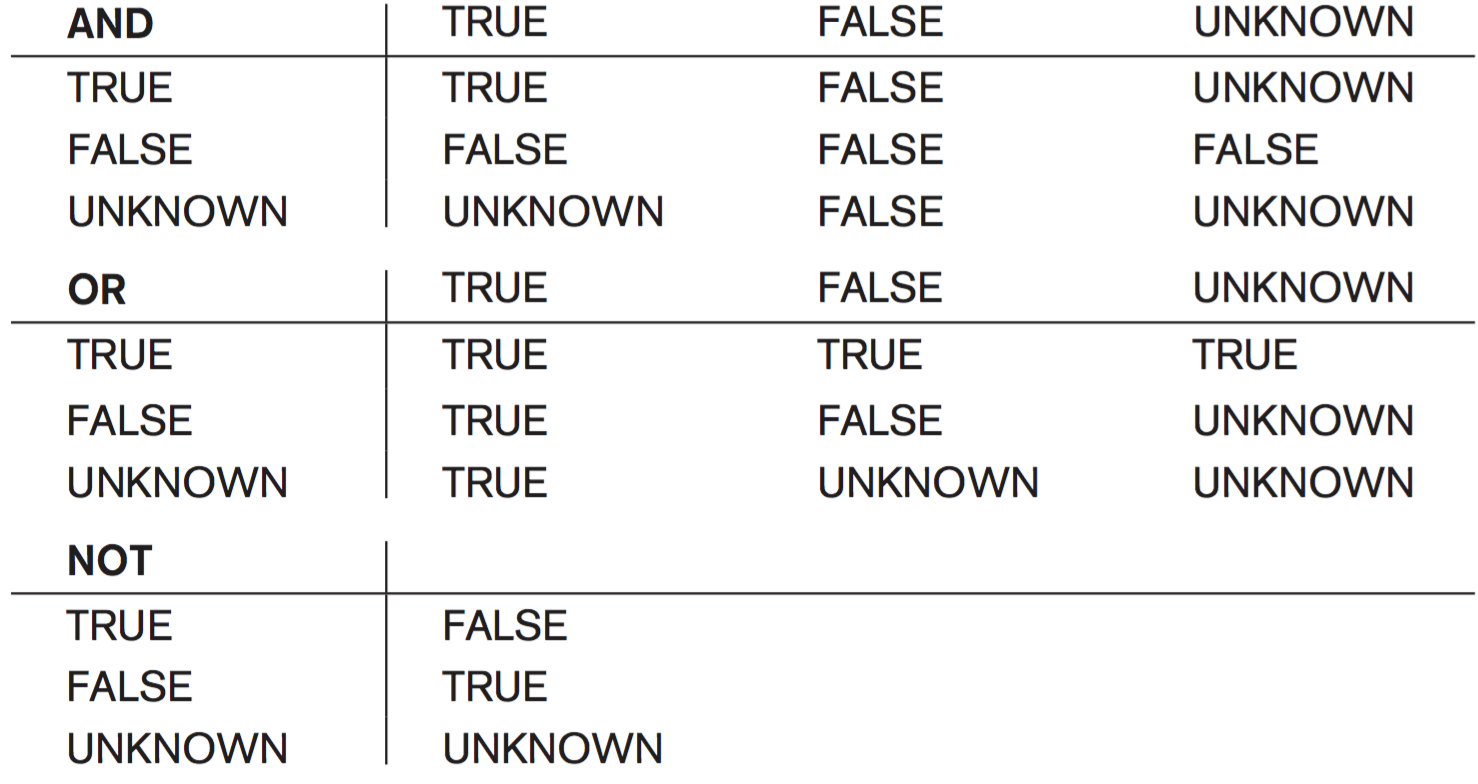
\includegraphics[scale = 0.5]{img/chap7-1}
    \caption{Logical table with \textbf{UNKNOWN}}
    \label{7-1}
\end{figure}
\textbf{UNKNOWN} is not kept in the result.
\subsection{Nested Queries, Tuples, and Set/Multiset Comparisons}
Some queries require that existing values in the database be fetched and then used in a comparison condition. To achieve it, we use Nested queries, they are complete \textit{SQL} requests within another \textit{SQL} query, called the outer query. The nested query can appear in any part of the outer query (\textbf{SELECT}, \textbf{FROM}, \textbf{WHERE}). We need to introduce the comparison operator \textbf{IN} which compare a value (or a tuple) with a set, return \textbf{TRUE} if the value is in the set.

If a nested query returns a single attribute and a single tuple, the query result will be a single value. In this case we can use "=" instead of \textbf{IN}. The = ANY (or = SOME) operator returns TRUE if the value is equal to some value in the set and is hence equivalent to \textbf{IN}. The keyword \textbf{ALL} can also be combined with each of these operators. These operators can be use with logical operators ($>,<, =, ...$)

\subsection{Correlated Nested Queries}
Whenever a condition in the \textbf{WHERE} clause of a nested query references some attribute of a relation declared in the outer query, the two queries are said to be correlated. We can understand a correlated query better by considering that the nested query is evaluated once for each tuple (or combination of tuples) in the outer query.
\subsection{The EXISTS and UNIQUE Functions in SQL}
\textbf{EXISTS} and \textbf{UNIQUE} are Boolean constraints to check if the result set of a nested query is empty or if it is unique, respectively. You can take the opposite with the keyword \textbf{NOT}

\subsection{Explicit Sets and Renaming in SQL}
You can use explicit set with \textbf{IN}. (...\textbf{WHERE} value \textbf{IN} (1,2,3 )).
You can rename what you want in \textbf{SELECT} and \textbf{FROM}. (The new name in \textbf{FROM} can be use in the corresponding \textbf{SELECT}).
\subsection{Joined Tables in SQL and Outer Joins}
You can join two tables with the instruction \textbf{JOIN ON}, that join two tables on an attribute. This instruction is done in the \textbf{FROM}. There is different type of \textbf{JOIN}:
\begin{itemize}
\item \textbf{NATURAL JOIN}: No join condition (no \textbf{ON}...), we can rename the result;
\item \textbf{INNER JOIN}: Default one, A tuple of a relation will be in the result only if it match a tuple in the other relation;
\item \textbf{OUTER JOIN}: There is a lot of different outer join: (\textbf{LEFT}(every tuple in the left table must appear in the result; if it does not have a matching tuple, it is padded with NULL values for the attributes of the right table), \textbf{RIGHT, FULL})
\item \textbf{CROSS JOIN}: Cartesian product.
\end{itemize}
\subsection{Aggregate Functions in SQL}
The aggregate functions, as \textbf{COUNT, SUM, MAX, MIN,} and \textbf{AVG} are used to summarize information and must be used in the \textbf{SELECT} statement. They return numeric values. You can refer to the row with * (\textbf{COUNT}(*) will return the number of row of the result query). Don't forget to use \textbf{DISTINCT} to discard duplicate results.
\subsection{Grouping: The GROUP BY and HAVING Clauses}
In many cases we want to apply the aggregate functions to subgroups of tuples in a relation, where the subgroups are based on some attribute values. We need to partition the relation in nonoverlaping subsets. Each subset will have the same value on the grouping attribute(s). We use \textbf{GROUP BY} to achieve it. The aggregate function will be computed for each subsets.

\textbf{HAVING} provides a condition on the summary information regarding the group of tuples associated with each value of the grouping attributes. Only the groups that satisfy the condition are retrieved in the result of the query, it must be use with \textbf{GROUP BY}.

\subsection{Other SQL Constructs: WITH and CASE}
\textbf{WITH} define a table that will only be used only in that query (quiet similar to a view). 

\textbf{CASE} can act differently due to different conditions, it can be usefull in an update operation for exemple. 
\textbf{UPDATE} table \textbf{SET} row = \textbf{CASE WHEN} condtion \textbf{THEN} ...
\subsection{Recursive Queries in SQL}
It's possible to specify recursive query in a declarative way. You may use \textbf{WITH RECURSIVE}.

\subsection{Discussion and Summary of SQL Queries}
It is possible to have six different clause in an \textit{SQL} query (\textbf{SELET, FROM, WHERE, GROUP BY, HAVING, ORDER BY}) but only \textbf{SELECT, FROM} are mandatory. 



\section{Specifying Constraints as Assertions and Actions as Triggers}
\subsection{Specifying General Constraints as Assertions in SQL}
In \textit{SQL}, we can specify general constraint (via declarative assertion) by using \textbf{CREATE ASSERTION}. Each assertion has a name and a condition (like in \textbf{WHERE}): \textbf{CREATE ASSERTION} name \textbf{CHECK} condition. The condition must be true for every database state to satisfy the assertion. The DBMS is responsible for ensur- ing that the condition is not violated.

The basic technique for writing such assertions is to specify a query that selects any tuples that violate the desired condition. By including this query inside a \textbf{NOT EXISTS} clause, the assertion will specify that the result of this query must be empty so that the condition will always be \textbf{TRUE}. Thus, the assertion is violated if the result of the query is not empty. 
\subsection{Introduction to Triggers in SQL}
Triggers are really important in \textit{SQL}, you can create them with \textbf{CREATE TRIGGER}. A trigger execute an action (a procedure or trigger other update) when a specify event appears. A trigger has three components:
\begin{itemize}
\item The event: specified by \textbf{BEFORE/AFTER INSERT/UPDATE OF };
\item The condition: determines whether the rule action should be executed (if no condition, it appears once the event appears), specified by \textbf{WHEN};
\item The action: it could be procedure, \textit{SQL} code, ...
\end{itemize}
Triggers can be used in various applications, such as maintaining database consistency, monitoring database updates, and updating derived data automatically.

\section{Views (Virtual Tables) in SQL}
\subsection{Concept of a View in SQL}
In \textit{SQL} a view is a virtual table derived from other tables taht can be real table or other views.
We can think of a view as a way of specifying a table that we need to reference frequently.

\subsection{Specification of Views in SQL}
We create a view this way: \textbf{CREATE VIEW} name[(columns names)] \textbf{AS} \textit{SQL} request. If the columns name are not specifier, they inherits the names of the attributes in the original table. A view is always up-to-date (done by DBMS). You can delete a view with \textbf{DROP VIEW} name.

\subsection{View Implementation, View Update, and Inline Views}
There is two approaches for the DBMS to implement an efficient view for querying:
\begin{itemize}
\item Query modification: modifying the view query onto queries on the base tables. Inefficient for hard requests (a lot of base table or view involved);
\item View materialization: Create physically a temporary/persistent view table, bit it needs to be up-to-date. Incremental update have been developed for this purpose, where the DBMS can determine what new tuples must be inserted, deleted, or modified in a materialized view table when a database update is applied to one of the defining base tables. There are different update: immediate, lazy (when we query on the view), periodic (may get a result that is not up-to-date).
\end{itemize}
In many case, querying \textbf{INSERT, DELETE, UPDATE} in a view isn't possible. In general, an update on a view defined on a single table without any aggregate functions can be mapped to an update on the underlying base table under certain conditions. If there is join it is often not possible for the DBMS to determine which of the updates is intended. Update a view is possible, if there is only one way to make the update in the base table.

\subsection{Views as Authorization Mechanisms}
We will use views to hide some information to unauthorized people. 

\section{Schema Change Statements in SQL}
\subsection{The DROP Command}
\textbf{DROP}can be used to drop named schema elements, tables, domains, types, or constraints. \textbf{DROP SCHEMA} drop an entire schema. There is two options parameters:
\begin{itemize}
\item \textbf{RESTRICT}: delete a schema only if it empty and a table only if there is no references in any constraints;
\item \textbf{CASCADE}: delete all the elements that have a reference to the one we want to drop.
\end{itemize}

\subsection{The ALTER Command}
For base tables, the possible alter table actions include adding or dropping a column (attribute), changing a column definition, and adding or dropping table constraints. If we add a column and no default rule is used, all the relation will have a \textbf{NULL} value.
To drop a column we must use \textbf{CASCADE} or \textbf{RESTRICT}.

\section{Summary}
In this chapter, we have described: \textbf{CREATE ASSERTION}, allows the specification of more general constraints on the database; 
\textbf{CREATE TRIGGER}, that create a trigger, piece of code launch when a specific action appears; \textbf{CREATE VIEW}, create virtual table, used for frequently used table or to give only the information allowed for users; \textbf{SQL ALTER TABLE} statement, which is used for modifying the database tables and constraints. The figure \ref{7-2} summarize all the \textit{SQL} possible type of requests.
\begin{figure}[H]
    \centering
    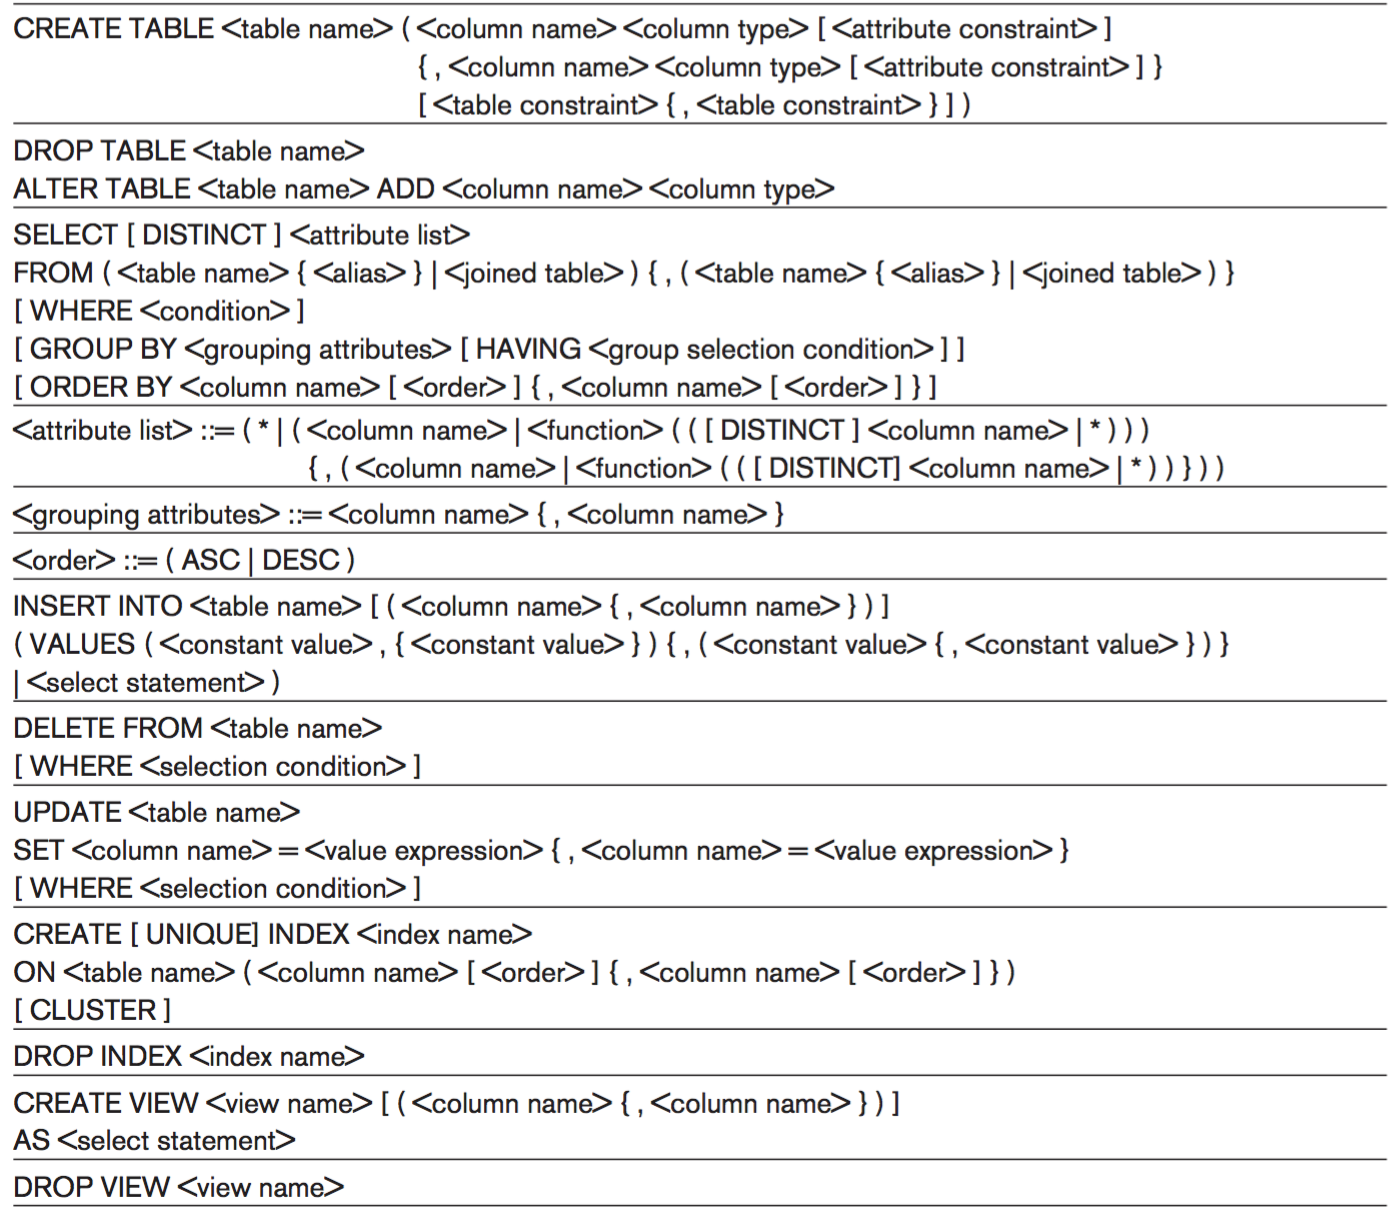
\includegraphics[scale = 0.5]{img/chap7-2}
    \caption{summary of \textit{SQL} requests.}
    \label{7-2}
\end{figure}



\chapter{Basics of Functional Dependencies and Normalization for Relational Databases (Chapter 14)}
The objective here is to formalize the notion of \textit{why one grouping of attributes may be better than another ?}. There are 2 levels to measure the goodness of a schema :
\begin{itemize}
    \item The logical (conceptual) level : What is the meaning of the attributes in the relation schema (base + views)
    \item The implementation (physical storage) level : How the tuples are stored and updated (only base)
\end{itemize}

There are 2 methods to deal with normalization :
\begin{itemize}
    \item Bottom-up : Consider the basic relationships and assemble them (not very popular)
    \item Top-down : Start with groupings of attributes, analyzed and decomposed
\end{itemize}
$\Rightarrow$ preserve information + minimum redundancy

\section{Informal Design Guidelines for Relation Schemas}
\subsection{Make sure that the semantics of the attributes is clear in the schema}
Attributes belonging to one relation have a real-world meaning and an interpretation with it.
\begin{center}
Easily explained semantic = better relation database schema
\end{center}

$\Rightarrow$\textbf{Guideline 1 } Design a relation schema so that it is easy to explain its meaning. Do not  combine attributes from various entity types into a single relation.


\subsection{Reduce the redundant information in tuples}
One aim is to minimize the storage used by the base relation. Let's take a look at figure \ref{fig:empdep} which shows two (natural) relations representing the list of employees and the list of departments. If we merge those two relations, we get the relation shown on figure \ref{fig:mixempdep}.\\

\begin{figure}[!h]
    \centering
    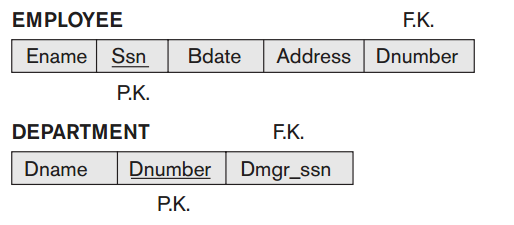
\includegraphics[scale=0.4]{chapter14_emp_dep.png}
    \caption{Employee-department, 2 relations (natural way)}
    \label{fig:empdep}
\end{figure}

\begin{figure}[!h]
    \centering
    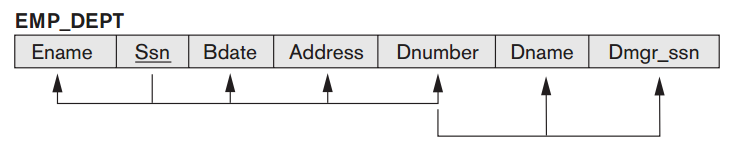
\includegraphics[scale=0.4]{chapter14_mix_emp_dep.png}
    \caption{Employee-department, mixed relations }
    \label{fig:mixempdep}
\end{figure}

In fact, what we will get by using the mixed version, is a severe redundancy of informations. For each employee, the Dname and Dmgr$\_$ssn will be repeated. It means that if 2000 employees are in the same department, the same combination of Dnumber/Dname and Dmgr$\_$ssn will appear 2000 times instead of 1 $\Rightarrow$ Huge redundancy $\Rightarrow$ huge loss of memory + possibility of update anomalies.
\newpage
\subsubsection{Update anomalies}
\begin{itemize}
    \item \textbf{Insertion anomalies} : When we add an employee and his department, we must be careful that all the values of this department are correct and consistent with the other tuples having this department number. Moreover, it is hard to add a department that has no employee. We must use NULL to achieve this.
    \item \textbf{Deletion anomalies} : If we delete the last employee of a certain department, then all informations about that department are lost.
    \item \textbf{Modification anomalies} : If we change the value of the manager of a department for example, we must update the tuples of all employee working for that department.\\
\end{itemize}
$\Rightarrow$\textbf{Guideline 2 } Design the database to limit the possibility of having insertion/deletion/modification anomalies. If you can't, notice clearly the programmer.

\subsection{Reduce the NULL values in tuples}
NULLs can cause several problems :
\begin{itemize}
    \item Waste space of storage level (large tables with lots of NULLs)
    \item Can cause problem with understanding the meaning of attributes after joins
    \item Problem with aggregate functions (count, sum,...)
    \item NULLs can have multiple significations :
    \begin{itemize}
        \item The attribute does not apply to the tuple
        \item The attribute value is unknown
        \item The attribute value is known but absent
    \end{itemize}
\end{itemize}
$\Rightarrow$\textbf{Guideline 3 } Avoid placing NULLable fields. If NULLs are unavoidable, make sure that they appear in exceptional cases.

\subsection{Disallowing the possibility of having spurious tuples}

Spurious tuples emerge from the splitting of a relation into several ones or from the mix of attributes from several relations. Its effect is to create new tuples when joining those new relations. The problem is that those new tuples are not supposed to hold, they are only here because of the join and the wrong design of the database.\\

$\Rightarrow$\textbf{Guideline 4 } Design relations schema so that they can be joined with equality conditions on attributes that are appropriately related (primary key, foreign key), in a way that guarantees that not spurious tuples are generated.

\section{Functional Dependencies}
\textbf{Definition} A functional dependency, denoted by X $\rightarrow$ Y, between two sets of attributes X and Y that are subsets of R specifies a constraint on the possible tuples that can form a relation state r of R. The constraint is that, for any two tuples t1 and t2 in r that have t1[X] = t2[X], they must also have t1[Y] = t2[Y] (X is called the left-hand side and Y the right hand side)\\

The main use of functional dependencies is to describe further a relation schema R by specifying constraints on its attributes that must hold at al times. Be careful, a FD is a property of the relation schema. Therefore, an FD cannot be inferred automatically from a given relation extension r, but must be defined explicitly by someone who knows the semantic of R. However, based on some FD, we can infer/deduce other functional dependencies.

\section{Normal Forms based on Primary Keys}
\subsection{Normalization of Relations}
The relation schema goes through a series of tests to certify if it satisfies a normal form (top down method). The aims of normalization are :
\begin{itemize}
  \item Minimize redundancy
  \item Minimize insertion, deletion and update anomalies
\end{itemize}

\begin{center}
\textbf{The normal form of a relation refers to the highest normal form
condition that it meets, and hence indicates the degree to which it has been
normalized}
\end{center}

In order to normalize properly, two properties must be respected :
\begin{itemize}
  \item Nonadditive join or lossless join property : No spurious tuble generation
  \item Dependency preservation property : Each FD is still present after decomposition\\
\end{itemize}

Be careful however that even if normalization is good, too much normalization can cause to increase the computational cost of some requests. Usually, we want to have 3NF or BCNF form, but 4-5-6NF are usually not necessary.

\subsection{Keys and Attributes participating in Keys}
Some definitions :
\begin{itemize}
\item \textbf{Superkey} of a relation schema R = \{$A_1$,$A_2$,...,$A_n$\} is a set of attributes S (included in R), with property that no two tuples $t_1$ and $t_2$ will have $t_1[S]$=$t_2[S]$.
\item \textbf{Key} K is a superkey with the property that removal of any attribute from K will cause K not to be a superkey anymore (a key has to be minimal)
\item \textbf{Candidate key} : If a relation schema has more than one key, each is called a candidate key
\item \textbf{Primary key} is a candidate key chosen arbitrarily as the primary key.
\item \textbf{Prime attribute} of R, is an attribute that is a member of at least one candidate key. The ones that are not prime are called \textbf{nonprime}
\end{itemize}

\subsection{First Normal Form}
\begin{center}
\textbf{The domain of an attribute must include only atomic values, and the value of any attribute in a tuple must be a single value from the domain of that attribute.}
\end{center}

There are 3 main methods to achieve 1NF :
\begin{enumerate}
  \item Remove the attribute that violates 1NF and place it in a separate relation, along with the corresponding primary key.
  \item Expand the key so that there will be a separate tuple in the original relation. The new primary key is then \{Old primary key,attribute causing trouble to 1NF\}. Problem = redundancy
  \item If a max number (k) of value is known for the attribute, replace the attribute by k attributes, and put null where no value fit. Problem : NULL values\\
\end{enumerate}
First normal form also disallow multivalued attributes that are themselves composite, also called nested relations (each tuple can have a relation within it). To remove this problem, consider that the primary key of the nested relation is called the partial key. Then, remove the nested relation attributes into a new relation and propagate the primary key into it. The primary key of this new relation will combine the primary key and the partial key. This procedure, called recursively is called unnesting.

\subsection{Second Normal Form}
First we need to introduce one new notion : \textbf{Full functional dependency}. A functional dependency X $\rightarrow$ Y is a full functional dependency if removal of any attribute A from X means that the dependency does not hold anymore. A functional dependency X $\leftarrow$ Y is a \textbf{partial dependency} if some attribute A $\in$ X can be removed from X and the dependency still holds.

\begin{center}
\textbf{A relation schema R is in 2NF if every nonprime attribute A in R is fully functionally dependent on the primary key of R}
\end{center}

\subsection{Third Normal Form}
\textbf{Transitive dependency} : Functional dependency X $\rightarrow$ Y, such that there exists a set of attributes Z $\in$ R that is neither a candidate key nor a subset of any key, and both X $\rightarrow$ Z and Z$\rightarrow$Y hold.

\begin{center}
\textbf{According to Codd’s original definition, a relation schema R is in 3NF if it satisfies 2NF and no nonprime attribute of R is transitively dependent on the primary key}
\end{center}

In order to solve that problem, as for 2NF, we need to decompose the original relation into new relations.

\section{General Definition of Second and Third Normal Forms}
Our definitions of 2NF and 3NF do not take all candidate keys into account for now, only the primary key. Now we will use the notion of prime attribute (defined above) and consider the partial/full/transitive dependencies with respect to all candidate keys.

\subsection{General definition of Second Normal Form}

\begin{center}
\textbf{A relation schema R is in second normal form (2NF) if every nonprime attribute A in R is not partially dependent on any key of R}
\end{center}

\subsection{General definition of Third Normal Form}

\begin{center}
\textbf{A relation schema R is in third normal form (3NF) if, whenever a
nontrivial functional dependency X $\rightarrow$ A holds in R, either 
\begin{itemize}
\item X is a superkey of R
\item A is a prime attribute of R
\end{itemize}
}
\end{center}

The second condition is our general definition of 3NF. However, the first condition catches two types of problematic dependencies :
\begin{itemize}
\item A nonprime attribute determines another nonprime attribute (transitive dependency that violates 3NF)
\item A proper subset of a key functionally determines a nonprime attribute (partial dependency that violates 2NF)

\end{itemize}


\section{Boyce-Codde Normal Form}
This normal form is stricter than 3NF.

\begin{center}
\textbf{A relation schema R is in BCNF if whenever a nontrivial functional dependency X $\rightarrow$ A holds in R, then X is a superkey of R}
\end{center}

In practice, most relation schemas that are in 3NF are also in BCNF. Only if there exists some f.d. X $\rightarrow$ A that holds in a relation schema R with X not being a superkey and A being a prime attribute will R be in 3NF but not in BCNF.\\

There are sometimes multiple possibilities of decomposing a relation so that it meets the BCNF requirements. Usually, what we will take the ones that respects \textit{the most} the two properties of decomposition :
\begin{itemize}
\item Nonadditive Join property
\item Functional dependency preservation property
\end{itemize}

In general, we can use this rule to decompose a non-BCNF relation :\\

Let R be the relation not in BCNF, let X a subset of attributes of R, and let X $\rightarrow$ A be the FD that causes a violation of BCNF. R may be decomposed into two relations:
\begin{itemize}
\item R-A
\item XA
\end{itemize}


\section{Multivalued Dependency and Fourth Normal Form}
\textbf{Definition} : A multivalued dependency X $\rightarrow \rightarrow$ Y specified on relation schema R, where X and Y are both subsets of R, specifies the following constraint on any relation state r of R: If two tuples $t_1$ and $t_2$ exist in r such that $t_1$[X] = $t_2$[X], then two tuples $t_3$ and $t_4$ should also exist in r with the following properties, where we use Z to denote (R - (X $\cup$  Y)).
\begin{itemize}
\item $t_1$[X] = $t_2$[X] = $t_3$[X] = $t_4$[X]
\item $t_3$[Y] = $t_1$[Y] and $t_4$[Y] =$t_2$[Y]
\item $t_3$[Z] =$t_2$[Z] and $t_4$[Z] = $t_1$[Z]  \\
\end{itemize}

A trivial MVD X $\rightarrow \rightarrow$ Y is one where Y is a subset of X or X $\cup$ Y = R. A MVD is said to be nontrivial if it respects none of both conditions. If we have a nontrivial MVD in a relation, we may have redundancy, which is undesirable.

\begin{center}
\textbf{A relation schema R is in 4NF with respect to a set of dependencies F (that includes functional dependencies and multivalued dependencies) if, for
every nontrivial multivalued dependency X $\rightarrow$
$\rightarrow$ Y in $F^+$ , X is a superkey for R}
\end{center}

In order to normalize this relation, we have to decompose it so that each MVD is represented by a separate relation where it becomes a trivial MVD.


\section{Join dependencies and Fifth Normal Form}
5NF present the notion of multiway decomposition into 5NF. Such a dependency is rarely observed and difficult to detect in practice, this is why 5NF is rarely done.\\

\textbf{Definition} : A join dependency (JD), denoted by JD($R_1$ , $R_2$ , ... , $R_n$ ), specified on relation schema R, specifies a constraint on the states r of R. The constraint states that every legal state r of R should have a nonadditive join decomposition into $R_1$ , $R_2$ , ... , $R_n$ . Hence, for every such r we have :
\begin{center}
* ($\pi _{R_1} $(r), $\pi _{R_2} $(r), ... , $\pi _{R_n} $(r)) = r
\end{center}

We can see that MVD is a special case of JD where n = 2. Based on the definition given above, we can define the $5^{th}$ normal form :
\begin{center}
\textbf{A relation schema R is in fifth normal form (5NF) (or project-join normal form (PJNF)) with respect to a set F of functional, multivalued, and join dependencies if, for every nontrivial join dependency JD($R_1$ , $R_2$ , ... , $R_n$ ) in $F^+$ (that is, implied by F), every R i is a superkey of R.}
\end{center}




\chapter{Disk Storage, Basic File Structures, Hashing, and Modern Storage Architectures (Chapter 16)}
%Flo
\section{Introduction}
Several types of storage can be used in a computer system~:
\begin{itemize}
    \item \textbf{Primary storage} can be operated on directly by the CPU. It includes main memory and small cache memories. These data are \textit{volatile}.
    \item \textbf{Secondary storage} is used for online storage. Magnetic disks are more and more replaced by SSDs.
    \item \textbf{Tertiary storage} includes optical disks and tapes. Used for offline storage (archives, ...).
\end{itemize}
Data must always be copied into primary storage before it can be processed by the CPU. \\

A database stored on disk is organized as \textbf{files} of \textbf{records}. Generally a DB is too large to fit entirely in main memory, so there are strategies to copy parts of it into main memory during a program execution.



\section{Secondary Storage Devices}

Disk devices are \textbf{random access} secondary storage because any block may be accessed at random while magnetic tapes are \textbf{sequential access} devices because $n$ blocks must be scanned to read block number $n$.

\subsubsection*{Hard Disk Drive}

An HDD is composed of several \textbf{cylinders}, each containing \textbf{tracks} of the same size, each containing \textbf{sectors} that contain \textbf{blocks}. The hardware mechanism that reads or writes a block is the \textbf{head} that contains a mechanical arm to move around the disk. \\

\begin{samepage}

The time to transfer a disk block is given by $s + r + b$ where
\begin{itemize}
    \item $s$ is the \textbf{seek time} = time to position the head on the right track
    \item $r$ is the \textbf{rotational delay} = time for the block to rotate into position under the head. It depends on the \textbf{rpm} of the disk. So in average $r=\dfrac{1}{2} \times \dfrac{1}{60 \times rpm}$.
    \item $b$ is the \textbf{block transfer time}
\end{itemize}
\end{samepage}

Usually $s$ and $r$ are much more significant than $b$. That is why it is common to transfer several consecutive blocks. \\

\subsubsection*{Solid-state Drive}

An SSD is a set of interconnected flash memory cards. Any address is directly addressable so the data is less likely to be fragmented. It is faster because no mechanical delay but also more expensive.

\subsubsection*{Magnetic Tapes}
The data blocks of a magnetic tapes are accessed in \textbf{sequential order}. Tape access can then be slow so their main function is \textbf{backing up} the DB.



\section{Placing File Records on Disk}

A file is a sequence of records. It is made up of \textbf{fixed-length} or \textbf{variable-length} records. These records \textit{may} be of the same type.

\subsubsection*{Separating records}

For fixed-length records there is no need of separator. For variable-length records we can use a \textbf{separator} to place between records. Or one can give record lengths or offsets in block header. Also, in a file that includes records of different types, each record is preceded by a \textbf{record type} indicator.

\subsubsection*{Spanned records}

\begin{samepage}

Two main record organizations exist~:
\begin{itemize}
    \item \textbf{unspanned} : a record must be within one block. Much simpler but may waste space.
    \item \textbf{spanned} : a record can span over several blocks. Essential if record size > block size.
\end{itemize}
\end{samepage}

Figures~\ref{fig:chap16-unspanned} and~\ref{fig:chap16-spanned} show both strategies.

\begin{figure}[h]
    \centering
    \begin{subfigure}[b]{\linewidth}
        \centering
        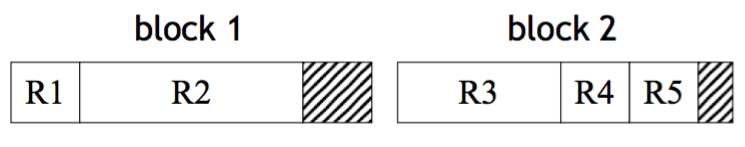
\includegraphics[scale=0.4]{chap16-unspanned.png}
        \caption{Unspanned}
        \label{fig:chap16-unspanned}
    \end{subfigure}
    
    \begin{subfigure}[b]{\linewidth}
        \centering
        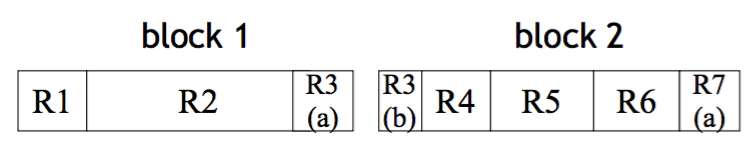
\includegraphics[scale=0.4]{chap16-spanned.png}
        \caption{Unspanned}
        \label{fig:chap16-spanned}
    \end{subfigure}
    \caption{Type of record organizations}
\end{figure}


\subsubsection*{Allocating File Blocks on Disk}
Two main techniques~:
\begin{itemize}
    \item \textbf{Contiguous allocation}~: file blocks are allocated to consecutive disk blocks. File expansion is hard but reading is very fast with double buffering.
    \item \textbf{Linked allocation}~: each file block contains a pointer to the next file block. Easy expand but slower reading.
\end{itemize}

Combinations of those two techniques are common such as \textbf{clustering} or \textbf{indexed allocation} or even combinations of these two.

\section{Operations on Files}
One access records in a file using a set of commands. Usually the program maintains a pointer to the current file record. The main commands are \textbf{open} and initialize a file, \textbf{find} a record matching a condition, \textbf{findnext} to iterate, \textbf{read} the file in a variable, \textbf{insert} a record, \textbf{delete} a record, \textbf{modify} a record, \textbf{close} the file, \textbf{reorganize} the file records, \textbf{read\_ordered} to read the records in a specific order.

\section{Various kinds of files}

\subsubsection*{Heap files}
Those are \textbf{unordered} files. Insertion is made at then end of the file and so is very efficient. But looking for a record is a \textit{linear search}.

\subsubsection*{Sorted files}
The records and the blocks in these files are \textbf{ordered} by some key value. Looking for a record is a \textit{binary search} but \textbf{only} if we access a record based on the key value. For other values it is a linear search. Record insertion and deletion are expensive because the records must remain ordered.

\subsubsection*{Hash files}
The search condition is an equality condition on a single field~: the \textbf{hash field}. The \textbf{hash function} is applied to the hash field value of a record $r$ and yields the address of the disk block in which $r$ is stored. Two main techniques exist~:

\begin{itemize}
    \item \textbf{Internal hashing} is implemented with a \textbf{hash table} and an array of records of length $M$. Then we have $M$ different values that the hash function can return.
    \item \textbf{External hashing} is implemented with \textbf{buckets}, each of which holds multiple records. The hashing function maps a key into a relative bucket.
\end{itemize}

In both cases \textbf{collision} may happen. It is less severe in external hashing because several records may fit in one bucket.

\chapter{Indexing Structures for Files and Physical Database Design (Chapter 17)}
% Indexes are used to \textbf{speed up} the retrieval of records in response to certain search conditions. The index are stored on disk and provide ways to access the records \textbf{without affecting their physical placement} on the disk. Any field of the file can be used to create an index. A variety of indexes are possible; each of them uses a particular data structure to speed up the search. To find a record or records in the data file based on a search condition on an indexing field, the index is searched, which leads to \textbf{pointers} to one or more disk blocks in the data file where the required records are located. 
\begin{itemize}
    \item An index is an auxiliary file that makes it more efficient to search for records in the data file.
    \item Usually specified on one field of the file, but could be more.
    \item The index file usually occupies considerably less disk blocks than the data file because its entries are much smaller
    \item A binary search on the index yields a pointer to the file record
    \item 
\end{itemize}

\section{Types of Single-Level Ordered Indexes}

An ordered index is similar to an index found at the end of a book. It lists important terms in some defined order (ex: alphabetical) along with the list of pages where the term appears (allows binary search). The alternative (without an index) would be to go page by page in the book to find the requested term (slow !).

For a file with a given record structure consisting of several attributes, an index is defined on a single attribute called \textbf{indexing attribute}.

An index is somewhat similar to dynamic hashing, except that the index search uses the value of the field itself, and not the hashing function's value on that field.

\begin{itemize}
    \item Dense index: there is an index value for each record in the data
    \item Sparse index: there is an index value for some record in the data
\end{itemize}


\begin{table}[]
    \centering
        \begin{tabular}{c|p{5cm}|p{5cm}}
            & Index Field Used for Physical Ordering of the File & Index Field Not Used for Physical Ordering of the File\\\hline
            Indexing field is key & Primary index & Secondary index (Key) \\
            Indexing field is non key & Clustering index & Secondary index (Non Key)\\
        \end{tabular}
    \caption{Comparison of indexes}
    \label{tab:indexesCMP1}
\end{table}


\begin{table}[]
    \centering
        \begin{tabular}{c|p{3cm}|p{3cm}|p{3cm}}
            Type & \# entries & Dense or Nondense(sparse) & Block anchoring on the data file\\\hline
            Primary & \# blocks in data file & Nondense & Yes\\
            Clustering & \# distinct index field values & Nondense & Yes/No\\
            Secondary(key) & \# records in data file & Dense & No\\
            Secondary (nonKey) & \# records or \# distinct field values & Dense or NonDense & No
        \end{tabular}
    \caption{Comparison of indexes}
    \label{tab:indexesCMP2}
\end{table}




\subsection{Primary Indexes}
Ordered file whose records are $<$ Primary key, Block anchor $>$. 
\begin{itemize}
    \item The file records on disk are \textbf{physically ordered} by the primary key, the primary key is thus an \emph{ordering key field}.
    \item There is one index entry \textbf{for each block} in the data file. 
    \item Each index entry has the value of the primary key field for the \textbf{first} record in a block.
    \item The first record of the data file is called the \textbf{anchor record} of the block, or \textbf{block anchor}
\end{itemize}

\paragraph{Insertion and deletion of records}
When inserting a record, we must:
    \begin{enumerate}
        \item Move records to make space for it
        \item Update the index of some entries, because moving records changes anchor records of some blocks
    \end{enumerate}
Reduce the problem by using an unordered overflow file, or a linked list of overflow records for each block in the data file.    

Note that only one primary index may exist, since you can't physically order the data in two different ways.

\subsection{Clustering Indexes}
If the file is physically ordered on a non-key field, that field is called \textbf{clustering field}. A clustering index is also an ordered file whose records are $<$ Clustering field, Disk block pointer$>$.
\begin{itemize}
    \item The file records on disk are physically ordered on the clustering field
    \item There is one entry for each \emph{distinct} value of the clustering field
    \item Each entry contains a pointer to the \emph{first block} in the data that has a record with that value for its clustering field
\end{itemize}
Note that only one clustering index may exist, since you can't physically order the data in two different ways.

One file may only have one clustering index OR one primary index, but not both. 

We could use block anchoring if every distinct value of the ordering field starts a new block.

\paragraph{Insertion and deletion of records}
Still poses problems because the data records are physically ordered. Reduce the problem by reserving a whole block (or a cluster of contiguous blocks) for each value of the clustering field.


\subsection{Secondary Indexes}
A data file can have several secondary indexes in addition to a clustering or primary index.

The field of the index record may be a \emph{non-ordering} \textbf{unique} value or a \textbf{duplicate} value in the data records.
The index is an ordered file whose records are $<$Field, block$|$record pointer$>$. We can't use block anchors, because the data file is not physically ordered by values of the field. 
There are 2 cases:
\begin{itemize}
    \item The field is \textbf{unique}
    \begin{itemize}
        \item One entry per record
        \item Dense index
    \end{itemize}
    \item The field is \textbf{not unique}: Numerous records in the data file can have the same value for the indexing field. Options to implement such an index are:
    \begin{enumerate}
        \item Include \textbf{duplicate} index entries with the same block or record pointer. One entry per record, thus dense index. (binary search must be adapted)
        \item Keep a \textbf{list} of block/record pointers for each value. (binary search must be adapted)
        \item Have a \textbf{single entry} for each \emph{index field value}, but create an extra level of \textbf{indirection} to handle the multiple pointers. For an index entry $<$K,P$>$, the block pointer $P$ points to a block of record pointers (a set of them), which point to records with value $K$. Binary search must not be changed and insertion of new records is straightforward. This is the option generally used.
    \end{enumerate}


\section{Multi-Level indexes}
In a single ordered index file, we use binary search to divide the search space in half. The idea with multilevel indexes is to divide it in $n (=$ the fan-out) at each step. Values for the fan-out are in the order of $300$.
See figure \ref{fig:chap17-multilevel} for an example.
\begin{figure}
    \centering
    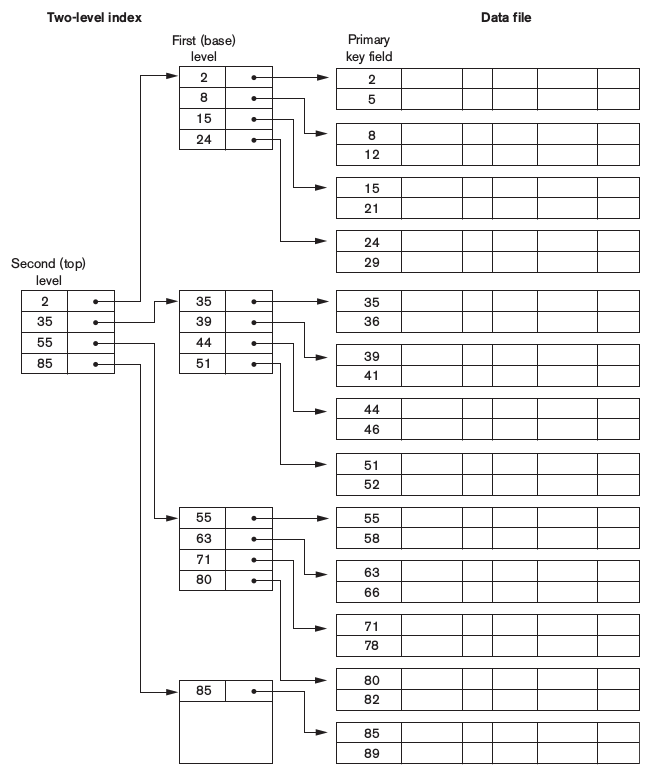
\includegraphics[scale=0.3]{chap17-1}
    \caption{A two-level primary index}
    \label{fig:chap17-multilevel}
\end{figure}

\paragraph{Insertion and deletion} use B-tree or B+-tree data structures. A node corresponds to a disk block, each node is kept between half full and completely full. We must keep the tree balanced on insertion and deletion.

\begin{itemize}
    \item Insertion
    \begin{itemize}
        \item Into a node that is not full is quite efficient
        \item If a node is full the insertion causes a split into
two nodes
        \item Splitting may propagate to other tree levels
    \end{itemize}
    \item Deletion
    \begin{itemize}
        \item Quite efficient if a node does not become less
than half full
        \item If causes a node to become less than half full,
it must be merged with neighboring nodes
    \end{itemize}
\end{itemize}

\begin{itemize}
    \item In a B-tree, pointers to data records exist
at all levels of the tree
    \item In a B+-tree, all pointers to data records
exists at the leaf-level nodes
    \item A B+-tree can have less levels (or higher
capacity of search values) than the
corresponding B-tree
\end{itemize}

Big chapter on B-tree etc... See book because not important.

\end{itemize}

\chapter{Strategies for Query Processing (Chapter 18)}

Steps taken to process an SQL query
\begin{enumerate}
    \item \textbf{Scan}: identify query tokens (key-words, attribute names, relation names)
    \item \textbf{Parser}: checks the syntax using grammar rules
    \item \textbf{Validation}: check that all attributes and relations are valid
    \item Internal representation of the query: \textbf{Query tree} or \textbf{Query graph (Directed acyclic graph)}
    \item \textbf{Query plan} + query \textbf{optimization}
\end{enumerate}

The \textbf{query optimizer} must produce a good execution plan, and the \textbf{code generator} generates the code to execute that plan. The \textbf{runtime database processor} has the task of running the query code to produce a query result. Figure \ref{fig:chap18-0}

\begin{figure}
    \centering
    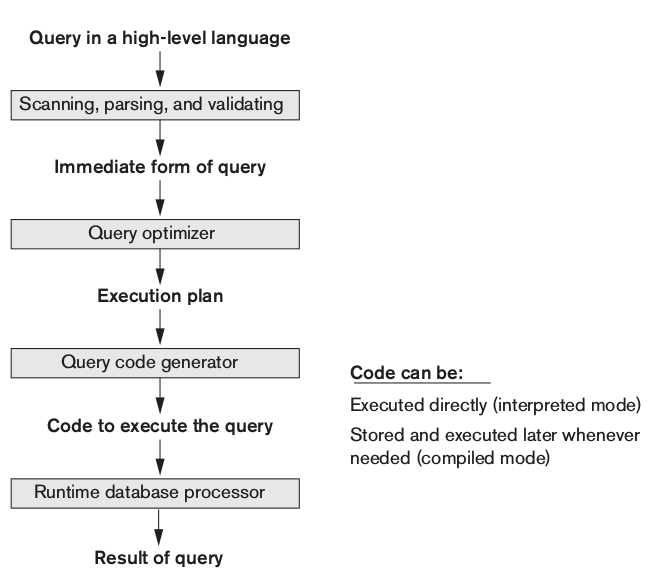
\includegraphics[scale=0.4]{chap18-0}
    \caption{Processing steps of a high-level query}
    \label{fig:chap18-0}
\end{figure}

\section{Translating SQL Queries into Relational
Algebra and Other Operators}

SQL queries are decomposed into \textbf{query blocks} which form the basic units that can be translated into the algebraic operators and optimized. A query block contains a single SELECT-FROM-WHERE expression (and optional GROUP BY and HAVING clauses). Figure \ref{fig:chap18-SQL-Rel}

\begin{figure}
    \centering
    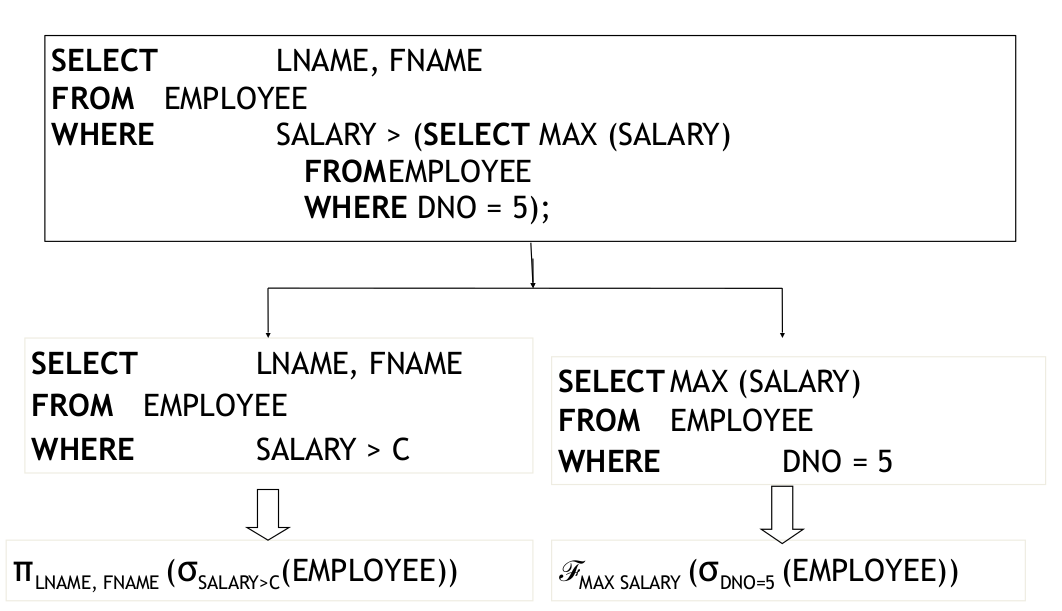
\includegraphics[scale=0.3]{chap18-1}
    \caption{SQL to relational algebra example}
    \label{fig:chap18-SQL-Rel}
\end{figure}

\begin{itemize}
    \item Select operation $\sigma_p(r)$ : Select $p$ from $r$. $p$ is a propositional logic expression
    \item Project operation $\prod_{A_1,...,A_n}(r)$ : projects columns $A_1,...,A_n$ from relation $r$
    \item Union Operation $r U s$: performs the union of relation r and s
    \item Set Difference $r - s$: tuples which are present in one relation but are not in the second relation.
    \item Cartesian Product $r X s$
    \item Rename Operation $\rho_x(E)$: the result of expression $E$ is saved with name of $x$.
\end{itemize}

%\section{Additional Operators Semi-Join and Anti-Join}
%Not important I think.

\section{Algorithms for External Sorting}
\begin{itemize}
    \item Sorting algorithms suitable for large files of records on disk
    \item Do not assume that data fit in main memory
    \item Is used for JOIN, ORDER-BY, etc...
    \item May be avoided by the use of an index.
\end{itemize}

\subsection{Sort-Merge strategy}
\begin{itemize}
    \item Sort small subfiles (runs) of the main file
    \item Merges sorted runs, creating larger sorted subfiles that are merged in turn
\end{itemize} 

\paragraph{Cost}
\begin{itemize}
    \item Sorting phase: Sorting the contents of exactly one disk block. $$nR = \ceil{b/nB}$$
    \item Merging phase: 
    $$dM = \min{(nB-1,nR)}$$
    $$nP= \ceil{\log_{dM}(nR)}$$
    \item Where \begin{itemize}
        \item nR: \# of initial runs
        \item b: \# of file blocks
        \item nB : available buffer space
        \item dM: degree of merging (number of sorted subfiles that can be merged in each merge step). During each merge step, one buffer block is needed to hold one disk block from each of the sorted subfiles being merged, and one additional buffer is needed for containing one disk block of the merge result
        \item nP: \# of passes
    \end{itemize}
\end{itemize}

\section{Algorithms for SELECT Operation}
SELECT = search operation to locate the records in a disk file that satisfy a certain condition. Different search algorithms are possible for selecting records from a file:
\begin{itemize}
    \item Linear search (brute force algorithm)
    \item Binary search (requires ordered file)
    \item Using a primary index or hash key (requires equality comparison on a key)
    \item Using a primary index to retrieve multiple records (requires comparison $>,\geq, <, \leq$ on a key). Use the index to find corresponding equality condition and retrieve all next or previous records in the ordered file.
    \item Using a clustering index to retrieve multiple records (requires equality comparison on a non-key attribute)
    \item Using a secondary ($B^+$-tree) index on an equality comparison. Can be used to retrieve a single record if the indexing field is a key (has unique values) or to retrieve multiple records if the indexing field is not a key.
\end{itemize}

\begin{itemize}
    \item Condition with only one attribute
    \begin{itemize}
        \item If an access path exists, use its corresponding method. Otherwise use brute force.
    \end{itemize}
    \item Condition with more than one attribute
    \begin{itemize}
        \item Query optimization to choose the access path that retrieves the fewest records in the most efficient way 
    \end{itemize}
\end{itemize}

%\section{Estimating the Selectivity of a Condition}
% Skipped

\section{Implementing the JOIN Operation}
Many JOIN are either EQUIJOIN or NATURAL JOIN.
\begin{itemize}
    \item \textbf{two-way join}: join on two files
    \item \textbf{multiway join}: join on more than two files
\end{itemize}
Methods for implementing joins:
\begin{itemize}
    \item \textbf{Nested-loop join} (brute-force).
    \begin{verbatim}
        foreach(t in R)
            foreach(s in S)
                test if t[A]=s[B]
    \end{verbatim}
    
    \item \textbf{Index-based nested-loop join}
    \begin{verbatim}
        foreach(t in R)
            use index or hash to get all matching records s from S such that s[B]=t[A]
    \end{verbatim}
    
    \item \textbf{Sort-merge join} 
    \begin{itemize}
        \item R physically sorted on A
        \item S physically sorted on B
        \item Both files scanned in order of the join attributes
        \item Records of each file are scanned only once (unless both A and B are non-key attributes)
    \end{itemize}
    
    \item \textbf{Hash-join}
    \begin{enumerate}
        \item Records of R are hashed into different buckets (if size of R < size of S, otherwise start with S) (= partitioning).
        \item Records of S are then hashed with the same function, and check if they are present in the bucket (= probing). Only keep the values that were already in the bucket.
    \end{enumerate}
    
\end{itemize}

%\section{How Buffer Space and Choice of Outer-Loop File Affect Performance of Nested-Loop Join}
% Skipped

%\section{How the Join Selection Factor Affects Join Performance}
% Skipped

%\section{General Case for Partition-Hash Join}
% Skipped

% \section{Hybrid Hash-Join}
% Skipped

\section{Algorithms for PROJECT}
A PROJECT operation $\pi_{<attribute list>} (R)$ from relational algebra implies that after projecting R on only the columns in the list of attributes, any duplicates are removed by treating the result strictly as a set of tuples.

\begin{itemize}
    \item If kept attributes include a key of R: extract all tuples from R with only the values for the attributes in attribute list
    \item Otherwise, duplicate tuples must be removed (using sorting or hashing)
\end{itemize}

\section{Algorithms for SET}
\begin{itemize}
    \item INTERSECTION and UNION:
    \begin{itemize}
        \item Sort tuples from both relations on the same attributes
        \item Scan and merge both sorted files concurently
        \item Keep only the tuples that appear in both relations (only keep one for UNION, to have unique tuples)
    \end{itemize}
    \item DIFFERENCE (R-S):
    \begin{itemize}
        \item Keep only those tuples that appear in relation R but not in S
    \end{itemize}
\end{itemize}

% \section{Use of Anti-Join for SET DIFFERENCE (or EXCEPT or MINUS in SQL)}
% Skipped

% \section{Implementing Aggregate Operations and Different Types of JOINs}
% Skipped

% \section{Implementing Different Types of JOINs}
% Skipped

% \section{Combining Operations Using Pipelining}
% Skipped

% \section{Parallel Algorithms for Query Processing}
% Skipped

\chapter{Query Optimization (Chapter 19)}
The goal of query optimization is to select the \textbf{best possible} strategy for query evaluation. \\

However the chosen plan is not always optimal.

\section{Query Trees and Heuristics for Query Optimization}

Optimizations techniques that apply \textbf{heuristics} to modify the internal representation of a query to \textbf{improve its performances}.\\

\textbf{Steps}:

\begin{itemize}
    \item Scanner and parser generate a data structure that corresponds to an \textbf{initial query representation}
    \item Query is optimized according to \textbf{heuristics} to obtain an optimized query representation
    \item \textbf{Query execution plan} is generated to execute groups of operations
\end{itemize}

One of the main \textbf{heuristics} is to apply \textbf{SELECT} and \textbf{PROJECT} before \textbf{JOIN} (because they reduce the size of the file before the join). Reduce the size of \textbf{intermediate results}.\\

\textbf{Data structures}:
\begin{itemize}
    \item {Query tree} (cfr. figure \ref{fig:tree}) used to represent a \textbf{relation algebra} expression
    \item \textbf{Query graph} (cfr. figure \ref{fig:graph}) is used for \textbf{relational calculus expression}
\end{itemize}

\begin{figure}[!h]
    \centering
    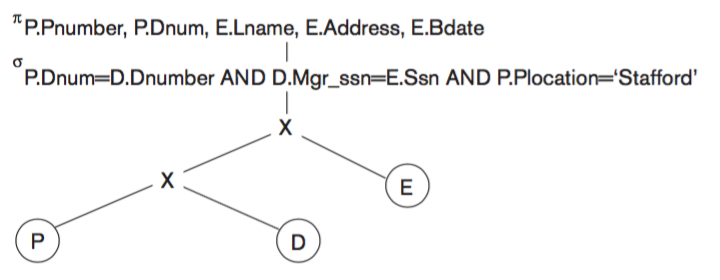
\includegraphics[scale=0.5]{chap19-1}
    \caption{Query tree}
    \label{fig:tree}
\end{figure}

\begin{figure}[!h]
    \centering
    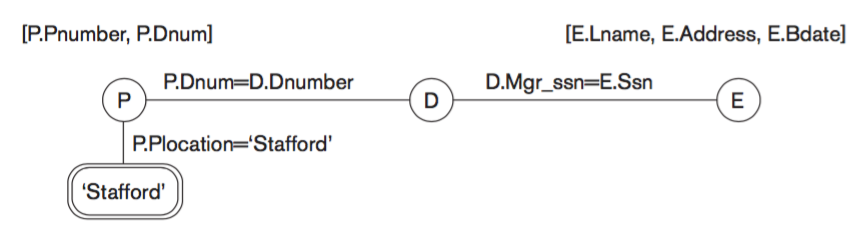
\includegraphics[scale=0.5]{chap19-2}
    \caption{Query graph}
    \label{fig:graph}
\end{figure}


\subsection{Notation for Query Trees and Query Graphs}

\textbf{Query tree} is composed of:

\begin{itemize}
    \item \textbf{Input relations} = leaves of the tree
    \item \textbf{Relational algebra operations} = internal nodes
\end{itemize}

\textbf{Execution} = execute an internal node whenever its operands are available.\\

\textbf{Query graph} is composed of:

\begin{itemize}
    \item \textbf{Input relations} = relations node (single circles)
    \item \textbf{Constant values} = constant nodes (double circles or ovals)
    \item \textbf{Selection and join conditions} = edges
\end{itemize}

\subsection{Heuristic Optimization of Query Trees}

Query parser first generates an initial query tree called \textbf{canonical query tree} but it might be very inefficient. So the \textbf{heuristic query optimizer} transforms it into a final query tree.\\

The optimizer includes rules of equivalence among relational algebra expression. \\

The list of the 16 transformation rules that can be applied can be found in the book at \textbf{page 698}. The most important ones are summarized below:\\

\begin{itemize}
    \item Cascade of SELECT and PROJECT
    \item Commutativity of SELECT, JOIN, UNION and INTERSECTION
    \item Associativity of JOIN, UNION and INTERSECTION
    \item Commuting PROJECT and RESTRICT
    \item Commuting RESTRICT and PROJECT
    \item Commuting RESTRICT and JOIN
    \item Commuting RESTRICT and SET Ops (UNION, INTERSECTION, MINUS)
    \item Commuting PROJECT and JOIN
    \item Commuting PROJECT and UNION
\end{itemize}

\textbf{Outline of a heuristic algebraic optimization algorithm}:
\begin{itemize}
    \item \textbf{Break up} any \textbf{SELECT} with conjunctive conditions into a cascade of SELECTS. It permits a greater degree of freedom in moving SELECT operations down the tree
    \item \textbf{Move} each \textbf{SELECT} as far down the tree as it is permitted by the attributes involved in the condition. If all the attributes are from the same table, move the SELECT to the leaf node for this relation. Otherwise move it where the corresponding tables are combined. 
    \item \textbf{Rearrange the leaf nodes}. Move the leaves with the most restrictive SELECT so they are executed first. Make sure that the ordering doesn't cause \textbf{Cartesian products}
    \item \textbf{Combine} cartesian product followed by a SELECT into a JOIN.
    \item \textbf{Move} the \textbf{PROJECT} as far as possible down the tree.
    \item \textbf{Identify} subgroups that can be executed by one algorithm
\end{itemize}

\textbf{Two approaches for evaluation}:

\begin{itemize}
    \item \textbf{materialized}: result of an operation is stored as a temporary result (physically materialized)
    \item \textbf{pipelined} (preferred): as resulting tuples are produced, they are forwarded directly to the next operation in the query sequence. 
\end{itemize}



\chapter{Introduction to Transaction Processing Concepts and Theory (Chapter 20)}
% Flo
\section{Introduction to Transaction Processing}
We consider here a \textbf{multiuser} DBMS. We then have concurrent accesses to the database. The model we treat in this chapter is \textbf{interleaved concurrency}~: the concurrent execution of processes is interleaved. It allows us to keep the CPU busy when a process requires an I/O operation. \\

A \textbf{transaction} is an executing program that forms a logical unit of database processing. It includes one or more database access operations. The transaction boundaries can be \textit{explicit} by specifying \textbf{begin transaction} and \textbf{end transaction} statements or \textit{implicit} because it is embedded within an application program. \\

The database model we consider is simplified. The DB is represented as a collection of \textit{named data items}. The size of a data item is called its \textbf{granularity}. A DB item can be an \textit{attribute value}, a \textit{database record} or a \textit{disk block} (in ascending granularity). \\

Basic database access operations that may be included in a transaction~:

\begin{itemize}
    \item \textbf{read\_item(X)}. Reads a DB item named X into a program variable, let us assume it is also named X.
    \item \textbf{write\_item(X)}. Writes the value of program variable X into the database item named X.
\end{itemize}

The \textbf{read-set} of a transaction T is the set of all items that T reads, and the \textbf{write-set} is the set of all items that T writes.

\subsection{Why Concurrency Control is Needed}
Different problems may occur if no concurrency control is used.

\begin{itemize}
    \item \textbf{The Lost Update Problem}. It occurs when two transactions accessing the same DB items have their operations interleaved such that the value of some DB items becomes incorrect. For instance $T_1$ changes the value of X and $T_2$ (that must occur after $T_1$) reads this value. If an interleaving yields a read of X by $T_2$ before $T_1$ has changed X, $T_2$ reads an incorrect value.
    
    \item \textbf{The Dirty Read Problem}. It occurs when $T_1$ updates X and then $T_1$ fails. Meanwhile, X is accessed by $T_2$ \textbf{before} X is rolled back because of the failure. $T_2$ then reads a \textit{dirty data}.
    
    \item \textbf{The incorrect Summary Problem}. It occurs when $T_1$ is calculating an aggregate summary function on a number of DB items while $T_2$ is updating some of these items. Wrong values are then aggregated by $T_1$.
    
    \item \textbf{The Unrepeatable Read Problem}. It occurs when $T_1$ reads two times a DB item X and $T_2$ updates the value of X between the two reads. 
\end{itemize}

\subsection{Why Recovery is Needed}
When a transaction $T$ is finished~:
\begin{itemize}
    \item if all the operations in $T$ are completed successfully, their effect is recorded permanently in the DB. This is a \textbf{commit}.
    \item Otherwise the operations in $T$ do not have any effect on the DB. This is an \textbf{abort}.
\end{itemize}

There are different types of failure that a DB can encounter.

\begin{itemize}
    \item Computer system crash
    \item Transaction error either because of system error or DB error (e.g. division by 0 or data not found).
    \item Concurrency control enforcement
    \item Physical problem such as disk failure, fire, explosion, Armageddon.
\end{itemize}

\section{Transaction and System Concepts}
A transaction $T$ can be in different states, as presented in figure~\ref{fig:chap20-transaction-states}. First $T$ is active to perform DB operations. When $T$ ends it is \textit{partially committed} and then is finally committed. If a problem occurs at any time before this point, $T$ fails. Eventually $T$ is terminated. In case of failure, $T$ must be \textbf{rolled back}, i.e. any changed that $T$ may have applied to the DB must be undone.

\begin{figure}[h!]
    \centering
    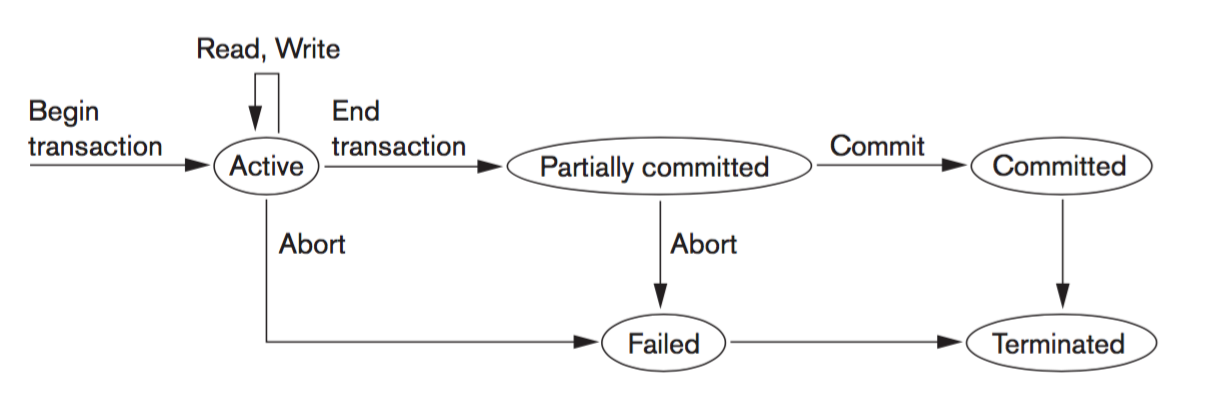
\includegraphics[scale=0.3]{chap20-transaction-states.png}
    \caption{State diagram illustrating the states for transaction execution}
    \label{fig:chap20-transaction-states}
\end{figure}

\subsection{The System Log}
The log is a sequential, append-only file kept on disk to keep track of all transaction operations. There are five possible actions to be recorded on the log.

\begin{itemize}
    \item \textbf{[start\_transaction, $T$]}. $T$ has started execution
    \item \textbf{write\_item, $T$, $X$, old\_value, new\_value}. $T$ has changed the value of $X$ from old\_value to new\_value.
    \item \textbf{read\_item, $T$, $X$}. $T$ has read the value of $X$.
    \item \textbf{commit, $T$}. $T$ has completed successfully and affirms that its effect can be committed to the DB.
    \item \textbf{abort, $T$}. $T$ has been aborted.
\end{itemize}

A transaction $T$ reaches its \textbf{commit point} when all its operations have been executed successfully and the effect of these operations have been recorded in the log.

\subsection{DBMS-Specific Buffer Replacement Policies}

A page replacement policy is needed when all the buffers in the DBMS cache are occupied and new disk pages are required to be loaded into main memory. Here are three of them.

\begin{itemize}
    \item \textbf{Domain Separation Method}. Each domain handles one type of disk page. Uses LRU, and so is static. Dynamic variant that adds load-balancing is Group LRU.
    \item \textbf{Hot Set Method}. Used for queries that have to scan a set of pages repeatedly, e.g. JOIN. This method determines which set of disk page is needed repeatedly.
    \item \textbf{The DBMIN Method}. Uses the Query Locality Set Model which determines the pattern of page references for each algorithm for a particular type of DB operation. Allocates right number of buffers using a locality set for each file.
\end{itemize}

\section{Desirable Properties of Transactions}
Transactions should possess the ACID properties~:

\begin{itemize}
    \item \textbf{Atomicity}. A transaction is atomic. Enforced by the \textit{transaction recovery subsystem}.
    \item \textbf{Consistency preservation}. It should takes the DB from one consistent state to another. The programmer is responsible for this.
    \item \textbf{Isolation}. Its execution should not interfer with other transactions executing concurrently. Enforced by the \textit{concurrency control subsystem}.
    \item \textbf{Durability}. Its changes to the DB must persist and must not be lost because of any failure. Enforced bu the \textit{recovery subsystem} of the DBMS.
\end{itemize}

\subsection{Levels of Isolation}
There are several levels of isolation of a transaction.

\begin{itemize}
    \item \textbf{Level 0} if it does not overwrite dirty reads of higher-level transactions.
    \item \textbf{Level 1} has no lost updates.
    \item \textbf{Level 2} has no lost updates nor dirty reads.
    \item \textbf{Level 3} as level 2, with repeatable reads in addition.
\end{itemize}


\section{Characterizing Schedules Based on Recoverability}
A \textbf{schedule} $S$ of $n$ transactions is an ordering of the operations of the transactions. We denote $r_i(X)$ and $w_i(X)$ a read and a write operation of transaction $i$ on data item $X$ respectively. \\

Two operations in a schedule are said to \textbf{conflict} if they satisfy all three of the following conditions~:
\begin{itemize}
    \item[1.] They belong to different transactions.
    \item[2.] They access the same data item $X$.
    \item[3.] At least one of the operations is $w(X)$.
\end{itemize}

A schedule $S$ is said to be a \textbf{complete schedule} if all three of the following conditions hold~:
\begin{itemize}
    \item[1.] The operations in $S$ are exactly those operations in $T_1$,...$T_n$, including a commit or abort operation as the last operation for each $T_i$ in $S$.
    \item[2.] For any pair of operations from the same $T_i$, their relative order of appearance in $S$ is the same as their order of appearance in $T_i$.
    \item[3.] For any two conflicting operations, one of the two must occur before the other in the schedule.
\end{itemize}
Condition 2 and 3 enforce a \textbf{total order} for any pair of conflicting operations and for any pair of operations from the same $T_i$ respectively. Nothing is required on non-conflicting operations not in the same transaction and so they follow a \textbf{partial order}.

\subsection{Characterizing Schedules Based on Recoverability}
A schedule $S$ is \textbf{recoverable} if no transaction $T$ in $S$ commits until all transactions $T'$ that have written some item $X$ that $T$ reads have committed. We said that $T$ reads from $T'$ if $X$ is first written by $T'$ and later read by $T$. \\

A schedule $S$ is \textbf{cascadeless} if every $T$ in $S$ reads only items that were written by committed transactions. \\

A schedule $S$ is \textbf{strict} if every $T$ can can neither read nor write an item $X$ until the last transaction that wrote $X$ has committed or aborted. \\

Suppose we have $n$ transactions $T_1, \dots ,T_n$. The set of \textit{all possible schedules} can be divided into two disjoint subsets~: recoverable and nonrecoverable. Also we have strict schedules $\subseteq$ cascadeless schedules $\subseteq$ recoverable schedules.

\begin{eqnarray*}
S_a &:& r_1(X); r_2(X); w_1(X); r_1(Y); w_2(X); c_2; w_1(Y); c_1; \\
S_b &:& r_1(X); w_1(X); r_2(X); r_1(Y); w_2(X); c_2; a_1;
\end{eqnarray*}

Let us consider the schedules $S_a$ and $S_b$ above where $c_i$ corresponds to the commit of $T_i$ and $a_i$ to the abort of $T_i$. Schedule $S_a$ is recoverable but $S_b$ is not. Indeed $T_2$ reads $X$ from $T_1$ but $T_2$ commits before $T_1$.

\section{Characterizing Schedules Based on Serializability}
A schedule $S$ is \textbf{serial} if for every $T \in S$ all the operations of $T$ are executed consecutively in $S$. We can make the assumption that every serial schedule is correct. The problem with these schedules is that it prevents any interleaving of operations. For instance if $T$ waits for an I/O operation we cannot switch the CPU to another $T'$. \\

A schedule $S$ is \textbf{serializable} if it is equivalent to some serial schedule. But how to define equivalence between schedules ? \\

Two schedules $S_1$ and $S_2$ are \textbf{result equivalent} if they produce the same final state of the database. The problem with this definition is that $S_1$ and $S_2$ may accidentally produce the same final DB state, as illustrated in figure~\ref{fig:chap20-result-equivalence}. Indeed if $X$ is 100 at the beginning, the two final DB states are identical. \\

\begin{figure}
    \centering
    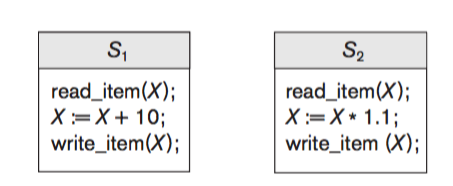
\includegraphics[scale=0.4]{chap20-result-equivalence.png}
    \caption{Result equivalence issue}
    \label{fig:chap20-result-equivalence}
\end{figure}

\textbf{Conflict Equivalence}. Two schedules are \textbf{conflict equivalent} if the relative order of any two conflicting operations is the same in both schedules. A direct consequence is that two conflict equivalent schedules yield the same final DB state. This definition is the more commonly used one. \\

\textbf{Conflict serializable Schedules}. A schedule $S$ is \textbf{conflict serializable} if it is conflict equivalent to some \textit{serial} schedule $S'$.


\subsection{Testing for Conflict Serializability of a Schedule}
There is a simple algorithm for determining wether a particular schedule is conflict serializable or not. However most concurrency control methods do \textit{not} test for conflict serializability. But this algorithm helps to understand the chapter on concurrency control protocols.\\

The algorithm constructs a \textbf{precedence graph} which is a directed graph $G=(N,E)$ where $N = \{T_1,\dots,T_n\}$ is the set of nodes and $E=\{e_1,\dots,e_m\}$ is the set of directed edges. \\

\textbf{Algorithm}
\begin{itemize}
    \item[1.] $\forall~T_i \in S$ create a node labeled $T_i$ in the precedence graph.
    \item[2.] For each case in $S$ where $T_j$ executes a DB operation after $T_i$ executes another DB operation where at least one of the two operations is a \texttt{write(X)}, create an edge ($T_i \rightarrow T_j$).
    \item[3.] $S$ is conflict serializable if and only if the precedence graph has no cycles.
\end{itemize}

Note that there is a directed edge ($T_i \rightarrow T_j$) if and only if a pair of conflicting operations exist in $T_i$ and $T_j$ and the one in $T_i$ appears in $S$ \textit{before} the one in $T_j$. Also, this edge means that $T_i$ must come before $T_j$ in any serial schedule equivalent to $S$. So if there is no cycle in the graph, we can create an equivalent serial schedule $S'$ by ordering the transactions in $S$ as described above.

\subsection{How Serializability is Used for Concurrency Control}
A \textit{serializable} schedule has an advantage over a \textit{serial} schedule~: it uses interleaving to use the CPU as much as possible. But testing for serializability is difficult and so DBMSs use \textbf{protocols} that ensures serializability of all schedules in which the transactions participate. Chapter~\ref{chap-concurrency-control} presents concurrency control protocols that guarantee serializability.


\subsection{View Equivalence and View Serializability}
Two schedules $S$ and $S'$ are \textbf{view equivalent} if the following three conditions hold~:

\begin{itemize}
    \item[1.] The same set of transactions participates in $S$ and $S'$.
    \item[2.] For any $r_i(X)$ in $S$, if the value of $X$ has been written by $w_j(X)$, the same condition must hold for the value of $X$ read by $r_i(X)$ in $S'$.
    \item[3.] If $w_k(Y)$ is the last \texttt{write} of $Y$ in $S$, then $w_k(Y)$ must also be the last \texttt{write} of $Y$ in $S'$.
\end{itemize}

The idea is that as long as each \texttt{read} operation reads the result of the same \texttt{write} operation in both schedules, the \texttt{write} operations of each transaction must produce the same results. \\

A schedule $S$ is \textbf{view serializable} if it is view equivalent to a \textit{serial} schedule. \\

Any conflict-serializable schedule is also view serializable. However, if there is no \textbf{blind write} both definition become equivalent. A \textbf{blind write} is a write operation in a transaction $T$ on an item $X$ that is not dependent on the old value of $X$, i.e. it is not preceded by a read of $X$ in $T$. For instance schedule $S_g$ defined below, $w_2(X)$ and $w_3(X)$ are blind writes.

$$S_g: r_1(X); w2_(X); w_1(X); w_3(X); c1; c2; c3;$$


\section{Transaction Support in SQL}
There is no explicit \texttt{Begin\_Transaction} in SQL to initiate a transaction. It is done implicitly when particular SQL statements are encountered. However, either a COMMIT or a ROLLBACK statement must end the transaction. Every transaction has 3 characteristics that may be specified~:

\begin{itemize}
    \item \textbf{Access mode} is READ ONLY or READ WRITE. Default mode is READ WRITE unless an isolation level of READ UNCOMMITTED is specified, then READ ONLY is assumed.
    \item \textbf{Diagnostic area size} is an integer $n$ that indicates the number of conditions held simultaneously in the diagnostic area. These supply feedback information for the user on the $n$ most recently executed SQL statements.
    \item \textbf{Isolation level} is READ UNCOMMITTED, READ COMMITTED, REPEATABLE READ or SERIALIZABLE. Default level is SERIALIZABLE. This is the highest level.
\end{itemize}

\begin{samepage}

If an isolation level different from SERIALIZABLE is specified, one or more of the following three violations may occur~:

\begin{itemize}
    \item[1.] \textbf{Dirty read}. $T_1$ reads the update of uncommitted transaction $T_2$, then $T_2$ aborts and so $T_1$ have read an incorrect value.
    \item[2.] \textbf{Nonrepeatable read}. $T_1$ reads a value from a table. $T_2$ then updates that value and $T_1$ reads that value again and so will see a different value.
    \item[3.] \textbf{Phantoms}. $T_1$ reads a set of rows from a table, say from a SQL WHERE-clause. Suppose $T_2$ inserts a new row $r$ in that table that also satisfies the WHERE-clause used in $T_1$. The record $r$ is called the \textbf{phantom record} because it was not there when $T_1$ starts but it is there when $T_1$ ends. $T_1$ may or may not see $r$.
\end{itemize}
\end{samepage}

Table~\ref{tab:chap20-isolation} summarizes the possible violations for the different isolation levels. A Yes means that the violation is possible. \\

\begin{table}[h!]
    \centering
    \bgroup
    \def\arraystretch{1.1}
    \begin{tabular}{llll}
         & & \textbf{Type of Violation} & \\\cline{2-4}
        \textbf{Isolation level} & \textbf{Dirty read} & \textbf{Nonrepeatable read} & \textbf{Phantom} \\
        READ UNCOMMITTED & Yes & Yes & Yes \\
        READ COMMITTED & No & Yes & Yes \\
        REPEATABLE READ & No & No & Yes \\
        SERIALIZABLE & No & No & No
    \end{tabular}
    \caption{Possible violations based on isolation levels}
    \label{tab:chap20-isolation}
    \egroup
\end{table}

\textbf{Snapshot Isolation}. This is another isolation level where a transaction $T$ sees the data items it reads based on the committed values of the items in the database state when $T$ starts. This ensures that the phantom record problem does not occur since $T$ will only see the records that were committed in the DB at the time it starts. A concurrency protocol based on this concept is presented in chapter~\ref{chap-concurrency-control}.

\chapter{Concurrency Control Techniques (Chapter 21)}
\label{chap-concurrency-control}
\section{Two-Phase Locking Techniques}
A lock is associated with each data item to control the access by concurrent transactions.

\subsection{Types of Locks and System Lock Tables}
\begin{description}
    \item [Binary locks:] Simple but too restrictive.\\
        2 states: locked (1) or unlocked (0).\\
        2 operations that can be called by a transaction: \texttt{lock\_item(X)} and \texttt{unlock\_item(X)}.\\
            lock\_item(X): if LOCK(X)=1, wait until LOCK(X)=0 (by putting the transaction in the waiting queue of item X). If LOCK(X)=0, then set LOCK(X)=1.\\
        Note that no interleaving should be allowed while these methods run.\\
        
        A \textbf{lock table} contains all the items that are locked. Each lock can be represented by the locked item, the locking transaction and a waiting queue containing transactions.
        
        Each transaction has to:
        \begin{itemize}
            \item call \texttt{lock\_item} before any read and write operation
            \item call \texttt{unlock\_item} after all read and write operations are completed in the transaction
            \item don't call \texttt{lock\_item} if already holds the lock
            \item don't call \texttt{unlock\_item} if it doesn't hold the lock
        \end{itemize}
        
        
    \item [Shared/Exclusive (or Read/Write) Locks:] More general. Read operations on the same item by different transactions are not conflicting. So we should allow several transactions to access the same item X if they all access X for reading purposes only.\\
    3 states: read-locked (=share-locked), write-locked (=exclusive-locked), or unlocked.\\
    3 operations: \texttt{read\_lock(X)}, \texttt{write\_lock(X)} and \texttt{unlock(X)}. Again, no interleaving is allowed.\\
    
    Implementation: the records of the lock table are of the form $<$Data\_item\_name, LOCK (read-locked or write-locked), Number\_of\_reads, locking\_transactions (a list)$>$. Unlock a read-locked lock only if Number\_of\_reads is 0.\\
    
    A transaction must call \texttt{write\_lock} if it performs a write operation and can call either \texttt{read\_lock} or \texttt{write\_lock} if it performs a read. But a transaction can't lock an item it already holds.
    
    \item [Conversion (Upgrading, Downgrading) of Locks:] A lock can be upgraded from read-locked to write-locked (by calling \texttt{write\_lock(X)}) if it is the only transaction holding the lock, otherwise the transaction must wait. A lock can be downgraded from write-locked to read-locked (by calling \texttt{read\_lock(X)}). This is why locking\_transactions is used in the lock table.
\end{description}

\subsection{Two-Phase Locking (2PL): Guarantees Serializability}
All locking operations precede the first unlock in the transaction.

2 phases: growing phase (new locks are acquired) and shrinking phase (locks are released).

If every transaction in a schedule follows the two-phase locking protocol, then the schedule is guaranteed to be serializable. A transaction schedule is serializable if its outcome is equal to the outcome of its transactions executed serially (sequentially without overlapping in time). This protocol limits the amount of concurrency that can occur in a schedule.\\

Variations of 2PL:
\begin{description}
    \item[conservative 2PL:] a transaction should lock all the items it accesses before the transaction begins its execution. It is a deadlock-free protocol but difficult to use in practice.
    \item[strict 2PL:] a transaction does not release any of its exclusive (write) locks before it terminates. Not deadlock-free.
    \item[rigorous 2PL:] a transaction does not release any of its locks (exclusive or shared) before it terminates.
\end{description}

\subsection{Dealing with Deadlock and Starvation}
Deadlock: each transaction is waiting for an item locked by another transaction.

Deadlock prevention protocols:
\begin{itemize}
    \item Every transaction lock all the items it needs in advance (used in conservative 2PL). Lock all the items or wait with no item locked.
    \item \textbf{Wait-die:} If TS(T1) $<$ TS(T2), then T1 is allowed to wait; otherwise (T1 younger than T2) abort T1 (T1 dies) and restart it later with the same timestamp.
    \item \textbf{Wound-wait:} If TS(T1) $<$ TS(T2), then abort T2 (T1 wounds T2) and restart it later with the same timestamp; otherwise (T1 younger than T2) T1 is allowed to wait.
    \item \textbf{No waiting algorithm:} if a transaction is unable to obtain a lock, it is immediately aborted and then restarted after a certain time delay.
    \item \textbf{Cautious waiting algorithm:} If T2 is not blocked (not waiting), then T1 is blocked and allowed to wait; otherwise abort T1.
\end{itemize}

Deadlock detection (alternative to prevention protocols):\\
\begin{description}
    \item[Wait-for graph:] 1 node/executing transaction, edge if a transaction is waiting for an item locked by another transaction. Deadlock if cycle in the graph. Abort some of the transactions in the cycle --$>$ Victim selection: better to choose younger transactions. 
    \item[Timeouts:] abort transaction if waiting for too long.
\end{description}

To avoid starvation: use a first-come-first-served queue, or higher priority to transactions waiting for a long time or being frequently aborted. Wait-die and wound-wai avoid starvation, because they restart an aborted transaction with its same timestamp.

\section{Concurrency Control Based on Timestamp Ordering}
Concurrency control techniques based on timestamp ordering do not use locks, so deadlocks cannot occur. The schedule is serializable. Tnterleavings of transaction operations are allowed, but for each pair of conflicting operations in the schedule, the order in which the item is accessed must follow the timestamp order. Each item X is associated with two values: read\_TS(X), the timestamp of the last transaction that read X, and write\_TX(X), the timestamps of the last transaction that have written X.
\begin{description}
    \item[Basic Timestamp Ordering:] if a transaction tries to write an item with a smaller (read or write) timestamp or tries to read an item with a smaller write timestamp, abort the transaction and rollback all the transactions that have used an item written by the aborted transaction, and rollback the transactions that have used an item written by the rollbacked transactions etc. (cascading rollback). Give a new timestamp when the transaction is restarted (not like in wait-die and wound-wait).
    \item[Strict Timestamp Ordering:] if read\_item(X) or write\_item(X) called: if TS(T) $>$ write\_TS(X) then wait until T' (the transaction that have written X) terminates. If write\_item(X) called:
    \begin{itemize}
        \item if read\_TS(X) $>$ TS(T): abort T.
        \item if write\_TS(X) $>$ TS(T): don't abort T but jump the write operation. (Remark that any conflict would have been avoided thanks to the first condition). 
        \item otherwise execute the write operation and set write\_TS(X) to TS(T).
    \end{itemize} 
\end{description}

\section{Multiversion Concurrency Control Techniques}
Keep copies of the old values of a data item when the item is written. The read operations can read an older version of an item instead of being rejected. This maintains serializability.

\subsection{Multiversion Technique Based on Timestamp Ordering}
Each version $X_i$ of an item keeps 2 timestamps: read\_TS($X_i$) and write\_TS($X_i$). Rules to ensure serializability: find the version i of X that has the highest write\_TS($X_i$) of all versions of X that is also less than or equal to TS(T), then
\begin{itemize}
    \item write operation: aborted if read\_TS($X_i$) $>$ TS(T) (because another transaction that should read after the write of T has already read this version). 
    \item read operation: return the value of $X_i$ and set read\_TS($X_i$) to the highest timestamp between TS(T) and the existing one.
\end{itemize}

\subsection{Multiversion Two-Phase Locking Using Certify Locks}
4 states: read-locked, write-locked, certify-locked, or unlocked.\\

The idea behind multiversion 2PL is to allow other transactions T' to read an item X while a single transaction T holds a write lock on X (which is not possible in the other schemes). A local version X' of an item is created each time a transaction acquires a write lock on X. Other transactions can continue to read the commited version of X. Once T is ready to commit its local version, it must obtain a certify lock on all items that it currently holds write locks on before it can commit. The certify lock is not compatible with read locks.

\section{Validation (Optimistic) Techniques and Snapshot Isolation Concurrency Control}
\subsection{Validation-Based (Optimistic) Concurrency Control}
No checking is done while the transaction is executing, so there is less overhead during execution. During transaction execution, all updates are applied to local copies of the data items. At the end, a validation phase checks whether any of the transaction’s updates violate serializability (all checks are done during this phase). Optimistic because it assumes that little interference will occur.\\

The validation phase for Ti checks that, for each such transaction Tj that is recently committed or in its validation phase, one of the following conditions holds to validate the transaction:
\begin{itemize}
    \item Tj completes its write phase before Ti starts its read phase.
    \item Ti starts its write phase after Tj completes its write phase, and the read\_set of Ti (the set of items it reads) has no items in common with the write\_set of Tj.
    \item The read\_set and write\_set of Ti have no item in common with the write\_set of Tj, and Tj completes its read phase before Ti completes its read phase.
\end{itemize}

\subsection{Concurrency Control Based on Snapshot Isolation}
The database transaction only sees the records that were committed in the database at the time the transaction started. Certain anomalies that violate serializability can occur when snapshot isolation is used as the basis for concurrency control. They are difficult to detect but rare (outside the scope of this book) so they have to be checked by the developer, not the DBMS.\\

Write locks are required but not read locks (better performance than 2PL if many reads).\\

To read the correct version of the item (so the version before the transaction started), keep the versions in a temporary version store with timestamps of when the version was created.

\section{Granularity of Data Items and Multiple Granularity Locking}
Granularity of the data items: what portion of the database a data item represents (field $<$ record $<$ disk block $<$ file $<$ whole database).

\subsection{Granularity Level Considerations for Locking}
The larger the data item size is, the lower the degree of concurrency is permitted: locking a whole disk block results in more conflicting transactions. Smaller data item size results in more locks and more locking operations performed.

\subsection{Multiple Granularity Level Locking}
Support multiple levels of granularity because the best granularity size depends on the given transaction. A transaction can choose the level to lock (a file, a record,...). A hierarchy tree is used to check if an item is locked: if transaction T1 is locking a whole file and T2 wants to lock a record in this file it has to traverse the tree to know if this record is locked.

Additional locks (from S (read/shared) and X (write/exclusive), intention locks, are needed:
\begin{description}
    \item[Intention-shared (IS)] indicates that read locks (shared locks) will be requested on some descendant nodes.
    \item[Intention-exclusive (IX)] indicates that write locks (exclusive locks) will be requested on some descendant nodes.
    \item[Shared-intention-exclusive (SIX)] indicates that the current node is locked in shared mode but that one or more exclusive locks will be requested on some descendant nodes.
\end{description}

Rules:
\begin{itemize}
    \item The root of the tree must be locked first, in any mode.
    \item A node N can be locked by a transaction T in S or IS mode only if the parent of node N is already locked by transaction T in either IS or IX mode.
    \item A node N can be locked by a transaction T in X, IX, or SIX mode only if the parent of node N is already locked by transaction T in either IX or SIX mode.
    \item A transaction T can lock a node only if it has not unlocked any node (to enforce the 2PL protocol).
    \item A transaction T can unlock a node N, only if none of the children of node N are currently locked by T.
\end{itemize}

So locking starts from the root to the node to be locked, unlocking starts from the locked node to the root.

\section{Other Concurrency Control Issues}
\subsection{Insertion, Deletion, and Phantom Records}
\textbf{Phantom record}. An example is better than long explanations:\\
Suppose that transaction T is inserting a new EMPLOYEE record whose Dno=5, whereas transaction T' is accessing all EMPLOYEE records whose Dno = 5 (for example to add up their salaries). Depending on the order of T and T', the new employee is included in the sum or not. But there is no real conflict because the record doesn't exist, so it can't be locked first (this problems occurs with insertion, not update).\\
Solution to the phantom record problem: use index locking or use predicate locking (lock access to all records that satisfy an arbitrary predicate).

\section{Summary}
The strict and rigorous variations are more common because of their better recoverability properties.\\

Locking can guarantee serializability when used in conjunction with the two-phase locking rule.\\

The timestamp ordering protocol ensures serializability based on the order of transaction timestamps.\\

Multiversion two-phase locking assumes that two versions can exist for an item and attempts to increase concurrency by making write and read locks compatible (at the cost of introducing an additional certify lock mode).\\

Snapshot isolation is used to lower overhead. The basic snapshot isolation method can allow nonserializable schedules in rare cases because of certain anomalies that are difficult to detect.\\

Multigranularity locking protocol allows the change of granularity (item size) based on the current transaction mix, with the goal of improving the performance of concurrency control.

\chapter{Database Recovery Techniques (Chapter 22)}
%Flo
\section{Recovery Concepts}

\subsection{Recovery Outline and Categorization of Recovery Algorithms}

Recovery from transaction failures means that the DB is restored to the most recent consistent state before the time of failure. To do this, the changes made by DB operations are kept in the \textbf{system log}. If there is extensive damage to a wide portion of the DB due to catastrophic failure, e.g. disk crash, the recovery method restores a past copy of the DB. Otherwise, the recovery strategy is to identify any changes that may cause inconsistency in the DB. \\

We distinguish between two main policies for recovery from non-catastrophic failures~:
\begin{itemize}
    \item \textbf{Deferred update} techniques update the DB only \textit{after} a transaction commits. These are discussed in section~\ref{chap22-deferred}.
    \item \textbf{Immediate update} techniques. The DB may be updated \textit{before} the transaction reaches its commit point. These are discussed in section~\ref{chap22-immediate}
\end{itemize}

Both techniques may involve UNDO and REDO operations. These apply to DB operations. They are \textbf{idempotent}, i.e. executing a specific operation multiple times is equivalent to executing it just once.

\subsection{Caching of Disk Blocks}
The \textbf{DBMS cache} is a collection of in-memory buffers. As the page tables in the operating system, there is a \textbf{directory} for the cache  to keep track of which items are in the buffers. Associated with each buffer is a \textbf{dirty bit}. As in the operating system it is used to denote a buffer that has been modified since its content has been brought from disk. Another bit is needed~: the \textbf{pin-unpin} bit. A page in the cache is \textbf{pinned} if it cannot be written back to disk as yet. It used by the recovery protocol to restrict certain buffer pages. \\

Two main strategies can be employed when flushing a modified buffer back to disk.

\begin{itemize}
    \item \textbf{In-place updating} writes the buffer to the \textit{same} original disk location, thus overwriting the old value.
    \item \textbf{Shadowing} writes the buffer at a \textit{different} disk location, thus multiple versions of the data item are kept on disk.
\end{itemize}

The old value of the data item before updating is called the \textbf{before image} (\textbf{BFIM}) and the new value after updating is called the \textbf{after image} (\textbf{AFIM}).


\subsection{Write-Ahead Logging, Steal/No-Steal, and Force/No-Force}
In an in-place updating scheme, the BFIM of the data item is recorded in the appropriate log entry and that log entry is flushed to disk before the BFIM is overwritten with the AFIM on disk. This process is called \textbf{write-ahead logging} and is necessary so we can UNDO the operation if needed. \\

\begin{samepage}
There are two types of log entry~:

\begin{itemize}
    \item \textbf{REDO-type log entry} includes the \textit{new} value AFIM of the item.
    \item \textbf{UNDO-type log entry} includes the \textit{old} value BFIM of the item.
\end{itemize}
\end{samepage}

If a cache buffer page updated by a transaction $T$ \textit{cannot} be written to disk before $T$ commits, the recovery method is called a \textbf{no-steal approach}. The pin-unpin bit is pinned. If the recovery protocol allows writing an updated buffer \textit{before} $T$ commits, it is called \textbf{steal}. Note that the \textit{no-steal} rule means that UNDO will never be needed during recovery. \\

If all pages updated by $T$ are immediately written to disk \textit{before} $T$ commits, the recovery protocol is called a \textbf{force approach}. Otherwise it is called \textbf{no-force}. Note that the \textit{force} rule means that REDO will never be needed during recovery. \\

\begin{samepage}
The \textbf{write-ahead logging} (\textbf{WAL}) protocol is used to permit recovery when in-place updating is used. It works as follows~:

\begin{itemize}
    \item[1.] The BFIM of an item $X$ cannot be overwritten by its $AFIM$ on disk until all UNDO-type log entries have been force-written to disk.
    \item[2.] The transaction $T$ cannot commit until all the REDO-type and UNDO-type log entries for $T$ have been force-written to disk.
\end{itemize}
\end{samepage}

\subsection{Checkpoints in the System Log and Fuzzy Checkpointing}
A \textbf{checkpoint} is a type of entry in the log, it is of the form \texttt{[checkpoint, \textit{list of active transactions}}. Taking a checkpoint consists of the following actions~:

\begin{itemize}
    \item[1.] Suspend execution of transactions.
    \item[2.] Force-write all main memory buffers that have been modified to disk.
    \item[3.] Write a [\texttt{checkpoint}] record to the log, and force-write the log to disk.
    \item[4.] Resume executing transactions.
\end{itemize}

To reduce the time during which transactions are suspended, the system can use \textbf{fuzzy checkpointing}. It consists of writing a \texttt{[begin\_checkpoint]} record at the beginning of step 2 and a \texttt{[end\_checkpoint]} record at the end of step 2. As soon as the first record is written, all transactions can be resumed.

\subsection{Transaction Rollback and Cascading Rollback}

If a transaction $T$ fails after updating the DB but before it commits, it may be necessary to \textbf{roll back} $T$. If $T$ is rolled back, any transaction $S$ that has read the value of some data item $X$ written by $T$ must also be rolled back. Similarly, once $S$ is rolled back, any transaction $R$ that has read the value of some data item $Y$ written by $S$ must also be rolled back, and so on. This phenomenon is called \textbf{cascading rollback}. However, almost all recovery mechanisms are designed so that cascading rollback is \textit{never required}. 


\section{NO-UNDO/REDO Recovery Based on Deferred Update}
\label{chap22-deferred}
A typical deferred update protocol can be stated as follows~:

\begin{itemize}
    \item[1.] A transaction $T$ cannot change the DB on disk until it reaches its commit point. Hence, all buffers that have been changed by $T$ must be pinned until $T$ commits. This is a \textit{no-steal} policy.
    \item[2.] A transaction $T$ does not reach its commit point until all its REDO-type log entries are recorded in the log \textit{and} the log buffer is force-written to disk. This is the WAL protocol.
\end{itemize}

So no UNDO is necessary since the DB is never updated on disk until after a transaction commits. A possible recovery algorithm using deferred update in a multiuser environment is the following~: \\

Use two lists of transactions~: the committed transactions $T$ since the \textit{last checkpoint} and the active transactions $T'$. REDO all the WRITE operations of the committed transactions from the log, \textit{in the order in which they were written into the log}. The transactions that are active and did not commit are effectively canceled and must be resubmitted. \\

\label{chap22-redo-proc}
\textbf{Procedure REDO (WRITE\_OP}~: Redoing a \texttt{write\_item} operation consists of examining its log entry [\texttt{write\_item},$T$,$X$,\texttt{new\_value}] and setting $X=\texttt{new\_value}$ in the DB. \\

Note that this protocol is more efficient if we start from the end of the log and redo only the \textit{last update} of each item $X$.

The advantage of this method is that transaction operations never need to be undone. Indeed, $T$ does not record any changes on disk until after it reaches its commit point and so $T$ is never rolled back. Also, $T$ will never read the value of an item that is written by an uncommitted transaction $T'$ so no cascading rollback will occur. \\

The drawback of this approach is that many cache buffers will be pinned and so cannot be replaced before the commit points of the transactions.



\section{Recovery Techniques Based on Immediate Update}
\label{chap22-immediate}
We can distinguish two main categories of immediate update algorithms. \\

\begin{itemize}
    \item[1.] All updates by a transaction $T$ are recorded on disk \textit{before} $T$ commits, so REDO is never needed. Hence this method uses the \textbf{steal/force} strategy.
    \item[2.] If $T$ is allowed to commit before all its changes are written to the DB, we have the general case, known as UNDO/REDO recovery algorithm. In this case, the \textbf{steal/no-force} strategy is applied. This is the most complex technique but also the most commonly used in practice.
\end{itemize}

The recovery procedure using immediate updates for a multiuser environment is presented below. However, we discuss in section~\ref{chap22-aries} a more practical approach known as ARIES.

\begin{itemize}
    \item[1.] Use two list of transactions~: the committed ones since the last \textit{checkpoint} and the active ones.
    \item[2.] Undo all the \texttt{write\_item} of the active transactions, using the UNDO procedure (showed below). They are undone in the reverse of the order in which they were written into the log.
    \item[3.] Redo all the \texttt{write\_item} of the committed transactions, using the REDO procedure (section~\ref{chap22-redo-proc}) in the order in which they were written into the log. 
\end{itemize}

\textbf{Procedure UNDO (WRITE\_OP)} consists of examining its log entry [\texttt{write\_item}, $T$, $X$, \texttt{old\_value}, \texttt{new\_value}] and setting $X=\texttt{old\_value}$.

Note that step 3, as presented for the NO-UNDO/REDO procedure is more efficiently done if we start from the end of the log and redo only the \textit{last update} of each item $X$.



\section{Shadow Paging}
In shadow paging, when a transaction $T$ begins, its \textbf{directory}, i.e. its $n$ cache entries that points to the most recent DB pages on disk, is copied into a \textbf{shadow directory}. During $T$ execution, the shadow directory is never modified. When a \texttt{write\_item} is performed, a new copy of the modified DB page is created~: the old page is not overwritten. Figure~\ref{fig:chap22-shadow} shows a situation during $T$ execution where pages 2 and 5 have been updated. \\

\begin{figure}[h!]
    \centering
    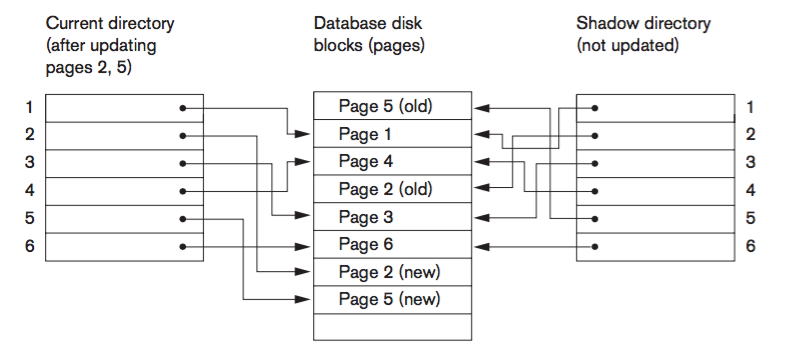
\includegraphics[scale=0.5]{chap22-shadow.png}
    \caption{An example of shadow paging}
    \label{fig:chap22-shadow}
\end{figure}

To recover from a failure during $T$ execution, we free the modified DB pages and discard the current directory. We then reinstate the shadow directory. To commit $T$, we discard the shadow directory. This is a NO-UNDO/NO-REDO technique for recovery. \\



\section{The ARIES Recovery Algorithm}
\label{chap22-aries}
ARIES is a specific scheme used in many of IBM’s relational database products. ARIES uses a steal/no-force approach for writing, and it is based on 3 concepts: \textbf{WAL, repeating history during redo, and logging changes during undo}.\\
\textbf{Repeating history}, means that ARIES will retrace all actions of the database system prior to the crash to reconstruct the database state when the crash occurred. Uncommitted transactions at the time of the crash are undone. \textbf{Logging during undo}, will prevent ARIES from repeating the completed undo operations if a failure occurs during recovery, which causes a restart of the recovery process.\\

The ARIES recovery procedure consists of three main steps: analysis (identity the dirty pages and set of transactions active at the time of the crash), REDO (not only applied to committed transaction: REDO all the logs from a start point to the end), and UNDO (operations of active transactions at the time of the crash are undone).\\

Every log record has an associated log sequence number (LSN) that is increasing and indicates the address of the log record on disk. A log record is written for any of the following actions: updating a page (write), committing a transaction (commit), aborting a transaction (abort), undoing an update (undo) (to avoid the undo to be repeated), and ending a transaction (end).\\

In addition to the log, two tables are needed for efficient recovery: the \textbf{Transaction Table} and the \textbf{Dirty Page Table}, both completed by the analysis phase. The REDO phase starts from the smallest LSN in the Dirty Page Table and proceeds up to the end of the log file. The Transaction Table contains the active transactions. The UNDO phase starts at the log entry from the latest active transaction and proceeds backwards in the log.\\

ARIES uses fuzzy checkpointing.

\section{Recovery in Multidatabase Systems}
A multidatabase transaction, may access to multiple databases. Each DBMS involved in the multidatabase transaction has its own recovery technique and transaction manager. To maintain the atomicity of a multidatabase transaction, it is necessary to have a two-level recovery mechanism: a global recovery manager and the local recovery managers. The global recovery manager usually follows the two-phase commit protocol:
\begin{itemize}
    \item \textbf{Phase 1.} Every local manager sends a message when it has finished the transaction and waits for the response of the global manager before committing. The global manager sends the response to all the local managers when they all said that they were ready to commit. Then the local managers reply with "ok" or "not ok" if it committed successfully of not.
    \item \textbf{Phase 2.} If a transaction has failed, then the global manager sends a message to rollback to all the local managers.
\end{itemize}
So all local databases commit the effect of the transaction or none of them do.

\section{Database Backup and Recovery from Catastrophic Failures}
The recovery techniques we have discussed use the entries in the system log or the shadow directory (both stored on disk) to recover from failure by bringing the database back to a consistent state. The recovery manager of a DBMS must also be equipped to handle more catastrophic failures such as disk crashes. Make frequent backups ! The system log should be backed up more frequently than the whole database to avoid losing all the effects of transactions that have been executed since the last backup. A new log is started after each database backup.

\section{Summary}
The main goal of recovery is to ensure the atomicity of a transaction. If a transaction fails before completing its execution, the recovery mechanism has to make sure that the transaction has no lasting effects on the database.\\

Deferred update techniques postpone the updating of the database on disk until a transaction reaches its commit point. The transaction force-writes the log to disk before recording the updates in the database. It never requires transaction rollback, and recovery simply consists of redoing the operations of transactions committed after the last checkpoint from the log. This leads to the NO-UNDO/REDO algorithm. In contrast, immediate update techniques, where changes to the database are applied on disk before the transaction commits, leads to the UNDO/REDO algorithm.\\

Shadow paging, classified as NO-UNDO/NO-REDO, does not require a log in single-user systems but still needs the log for multi-users systems.\\

Recovery from catastrophic failures is typically done by backing up the database and the log to tape. The log, which is backed up more frequently, can be used to redo operations starting from the last database backup.

\end{document}
